\documentclass[conference]{IEEEtran}
\IEEEoverridecommandlockouts
\usepackage[T1]{fontenc}
\usepackage{newtxtext,newtxmath}
\usepackage{amsmath}
\usepackage{graphicx}
\usepackage{booktabs}
\usepackage{xcolor}
\usepackage{cite}
\usepackage[hidelinks]{hyperref}
\graphicspath{{../results/figures/}}
% Generated by `python -m minesense.numbers` from results/. Do not edit.
\newcommand{\vRows}{338}
\newcommand{\vCountNoMine}{71}
\newcommand{\vCountAntiTank}{70}
\newcommand{\vCountAntiPersonnel}{66}
\newcommand{\vCountBoobyTrappedAP}{66}
\newcommand{\vCountMOneFourAP}{65}
\newcommand{\vGridObserved}{338}
\newcommand{\vGridCells}{360}
\newcommand{\vGridMissing}{22}
\newcommand{\vSaturatedRows}{18}
\newcommand{\vKaggleUciDiff}{5e-10}
\newcommand{\vTestFoldMin}{67}
\newcommand{\vTestFoldMax}{68}
\newcommand{\vTrainFirst}{229}
\newcommand{\vValFirst}{41}
\newcommand{\vSeriesNegativeRho}{30}
\newcommand{\vSeriesRhoBelow}{23}
\newcommand{\vEdaRTwoLinear}{0.859}
\newcommand{\vEdaRTwoCube}{0.896}
\newcommand{\vEdaDZero}{1.68}
\newcommand{\vEdaAllRTwoLinear}{0.876}
\newcommand{\vEdaAllRTwoCube}{0.876}
\newcommand{\vRTwoClass}{0.61}
\newcommand{\vRTwoClassHeight}{0.74}
\newcommand{\vRTwoAll}{0.76}
\newcommand{\vAccMlp}{0.648}
\newcommand{\vAccsdMlp}{0.055}
\newcommand{\vAccpctMlp}{64.8}
\newcommand{\vFOneMlp}{0.643}
\newcommand{\vDetMlp}{91.4}
\newcommand{\vDetsdMlp}{3.2}
\newcommand{\vMissMlp}{2.1}
\newcommand{\vFaMlp}{33.0}
\newcommand{\vAccminMlp}{55.9}
\newcommand{\vAccmaxMlp}{76.1}
\newcommand{\vAccMlpPhys}{0.667}
\newcommand{\vAccsdMlpPhys}{0.056}
\newcommand{\vAccpctMlpPhys}{66.7}
\newcommand{\vFOneMlpPhys}{0.661}
\newcommand{\vDetMlpPhys}{91.5}
\newcommand{\vDetsdMlpPhys}{2.9}
\newcommand{\vMissMlpPhys}{3.6}
\newcommand{\vFaMlpPhys}{27.1}
\newcommand{\vAccminMlpPhys}{58.8}
\newcommand{\vAccmaxMlpPhys}{79.4}
\newcommand{\vAccPiMlp}{0.676}
\newcommand{\vAccsdPiMlp}{0.062}
\newcommand{\vAccpctPiMlp}{67.6}
\newcommand{\vFOnePiMlp}{0.669}
\newcommand{\vDetPiMlp}{91.8}
\newcommand{\vDetsdPiMlp}{2.9}
\newcommand{\vMissPiMlp}{3.3}
\newcommand{\vFaPiMlp}{26.5}
\newcommand{\vAccminPiMlp}{55.9}
\newcommand{\vAccmaxPiMlp}{85.3}
\newcommand{\vAccFt}{0.692}
\newcommand{\vAccsdFt}{0.049}
\newcommand{\vAccpctFt}{69.2}
\newcommand{\vFOneFt}{0.682}
\newcommand{\vDetFt}{92.8}
\newcommand{\vDetsdFt}{3.1}
\newcommand{\vMissFt}{4.2}
\newcommand{\vFaFt}{18.6}
\newcommand{\vAccminFt}{61.8}
\newcommand{\vAccmaxFt}{77.6}
\newcommand{\vAccFtPhys}{0.691}
\newcommand{\vAccsdFtPhys}{0.059}
\newcommand{\vAccpctFtPhys}{69.1}
\newcommand{\vFOneFtPhys}{0.685}
\newcommand{\vDetFtPhys}{92.0}
\newcommand{\vDetsdFtPhys}{3.3}
\newcommand{\vMissFtPhys}{3.6}
\newcommand{\vFaFtPhys}{24.5}
\newcommand{\vAccminFtPhys}{58.8}
\newcommand{\vAccmaxFtPhys}{79.4}
\newcommand{\vAccPiFt}{0.703}
\newcommand{\vAccsdPiFt}{0.052}
\newcommand{\vAccpctPiFt}{70.3}
\newcommand{\vFOnePiFt}{0.693}
\newcommand{\vDetPiFt}{92.4}
\newcommand{\vDetsdPiFt}{2.9}
\newcommand{\vMissPiFt}{4.0}
\newcommand{\vFaPiFt}{20.9}
\newcommand{\vAccminPiFt}{58.8}
\newcommand{\vAccmaxPiFt}{83.8}
\newcommand{\vAccKnn}{0.439}
\newcommand{\vAccsdKnn}{0.055}
\newcommand{\vAccpctKnn}{43.9}
\newcommand{\vFOneKnn}{0.421}
\newcommand{\vDetKnn}{78.8}
\newcommand{\vDetsdKnn}{3.4}
\newcommand{\vMissKnn}{15.7}
\newcommand{\vFaKnn}{41.7}
\newcommand{\vAccminKnn}{36.8}
\newcommand{\vAccmaxKnn}{55.2}
\newcommand{\vAccSvm}{0.719}
\newcommand{\vAccsdSvm}{0.057}
\newcommand{\vAccpctSvm}{71.9}
\newcommand{\vFOneSvm}{0.706}
\newcommand{\vDetSvm}{93.1}
\newcommand{\vDetsdSvm}{2.9}
\newcommand{\vMissSvm}{5.8}
\newcommand{\vFaSvm}{11.3}
\newcommand{\vAccminSvm}{61.2}
\newcommand{\vAccmaxSvm}{80.6}
\newcommand{\vAccRf}{0.591}
\newcommand{\vAccsdRf}{0.048}
\newcommand{\vAccpctRf}{59.1}
\newcommand{\vFOneRf}{0.576}
\newcommand{\vDetRf}{90.6}
\newcommand{\vDetsdRf}{3.5}
\newcommand{\vMissRf}{7.3}
\newcommand{\vFaRf}{17.5}
\newcommand{\vAccminRf}{52.2}
\newcommand{\vAccmaxRf}{70.6}
\newcommand{\vAccXgb}{0.539}
\newcommand{\vAccsdXgb}{0.054}
\newcommand{\vAccpctXgb}{53.9}
\newcommand{\vFOneXgb}{0.523}
\newcommand{\vDetXgb}{88.6}
\newcommand{\vDetsdXgb}{4.2}
\newcommand{\vMissXgb}{8.5}
\newcommand{\vFaXgb}{22.4}
\newcommand{\vAccminXgb}{47.1}
\newcommand{\vAccmaxXgb}{64.2}
\newcommand{\vAccSvmNarrow}{0.728}
\newcommand{\vTuneMinPiFt}{8.3}
\newcommand{\vSvmCMedian}{6,545}
\newcommand{\vDiffPiFtVsKnnAccuracy}{26.5}
\newcommand{\vPwPiFtVsKnnAccuracy}{$<$\,0.001}
\newcommand{\vPtPiFtVsKnnAccuracy}{$<$\,0.001}
\newcommand{\vPthPiFtVsKnnAccuracy}{$<$\,0.001}
\newcommand{\vWinsPiFtVsKnnAccuracy}{25}
\newcommand{\vLossesPiFtVsKnnAccuracy}{0}
\newcommand{\vDiffPiFtVsKnnMacroFOne}{27.2}
\newcommand{\vPwPiFtVsKnnMacroFOne}{$<$\,0.001}
\newcommand{\vPtPiFtVsKnnMacroFOne}{$<$\,0.001}
\newcommand{\vPthPiFtVsKnnMacroFOne}{$<$\,0.001}
\newcommand{\vWinsPiFtVsKnnMacroFOne}{25}
\newcommand{\vLossesPiFtVsKnnMacroFOne}{0}
\newcommand{\vDiffPiFtVsKnnMineMissed}{11.7}
\newcommand{\vPwPiFtVsKnnMineMissed}{$<$\,0.001}
\newcommand{\vPtPiFtVsKnnMineMissed}{$=$ 0.0023}
\newcommand{\vPthPiFtVsKnnMineMissed}{$=$ 0.0091}
\newcommand{\vWinsPiFtVsKnnMineMissed}{0}
\newcommand{\vLossesPiFtVsKnnMineMissed}{25}
\newcommand{\vDiffPiFtVsKnnFalseAlarm}{20.8}
\newcommand{\vPwPiFtVsKnnFalseAlarm}{$<$\,0.001}
\newcommand{\vPtPiFtVsKnnFalseAlarm}{$=$ 0.018}
\newcommand{\vPthPiFtVsKnnFalseAlarm}{$=$ 0.072}
\newcommand{\vWinsPiFtVsKnnFalseAlarm}{0}
\newcommand{\vLossesPiFtVsKnnFalseAlarm}{22}
\newcommand{\vDiffPiFtVsSvmAccuracy}{1.6}
\newcommand{\vPwPiFtVsSvmAccuracy}{$=$ 0.33}
\newcommand{\vPtPiFtVsSvmAccuracy}{$=$ 0.66}
\newcommand{\vPthPiFtVsSvmAccuracy}{$=$ 0.66}
\newcommand{\vWinsPiFtVsSvmAccuracy}{9}
\newcommand{\vLossesPiFtVsSvmAccuracy}{13}
\newcommand{\vDiffPiFtVsSvmMacroFOne}{1.3}
\newcommand{\vPwPiFtVsSvmMacroFOne}{$=$ 0.41}
\newcommand{\vPtPiFtVsSvmMacroFOne}{$=$ 0.73}
\newcommand{\vPthPiFtVsSvmMacroFOne}{$=$ 0.73}
\newcommand{\vWinsPiFtVsSvmMacroFOne}{12}
\newcommand{\vLossesPiFtVsSvmMacroFOne}{13}
\newcommand{\vDiffPiFtVsSvmMineMissed}{1.7}
\newcommand{\vPwPiFtVsSvmMineMissed}{$=$ 0.0073}
\newcommand{\vPtPiFtVsSvmMineMissed}{$=$ 0.27}
\newcommand{\vPthPiFtVsSvmMineMissed}{$=$ 0.27}
\newcommand{\vWinsPiFtVsSvmMineMissed}{5}
\newcommand{\vLossesPiFtVsSvmMineMissed}{16}
\newcommand{\vDiffPiFtVsSvmFalseAlarm}{9.6}
\newcommand{\vPwPiFtVsSvmFalseAlarm}{$<$\,0.001}
\newcommand{\vPtPiFtVsSvmFalseAlarm}{$=$ 0.089}
\newcommand{\vPthPiFtVsSvmFalseAlarm}{$=$ 0.27}
\newcommand{\vWinsPiFtVsSvmFalseAlarm}{19}
\newcommand{\vLossesPiFtVsSvmFalseAlarm}{2}
\newcommand{\vDiffPiFtVsRfAccuracy}{11.2}
\newcommand{\vPwPiFtVsRfAccuracy}{$<$\,0.001}
\newcommand{\vPtPiFtVsRfAccuracy}{$<$\,0.001}
\newcommand{\vPthPiFtVsRfAccuracy}{$=$ 0.0017}
\newcommand{\vWinsPiFtVsRfAccuracy}{24}
\newcommand{\vLossesPiFtVsRfAccuracy}{0}
\newcommand{\vDiffPiFtVsRfMacroFOne}{11.7}
\newcommand{\vPwPiFtVsRfMacroFOne}{$<$\,0.001}
\newcommand{\vPtPiFtVsRfMacroFOne}{$=$ 0.0012}
\newcommand{\vPthPiFtVsRfMacroFOne}{$=$ 0.0024}
\newcommand{\vWinsPiFtVsRfMacroFOne}{25}
\newcommand{\vLossesPiFtVsRfMacroFOne}{0}
\newcommand{\vDiffPiFtVsRfMineMissed}{3.2}
\newcommand{\vPwPiFtVsRfMineMissed}{$<$\,0.001}
\newcommand{\vPtPiFtVsRfMineMissed}{$=$ 0.099}
\newcommand{\vPthPiFtVsRfMineMissed}{$=$ 0.20}
\newcommand{\vWinsPiFtVsRfMineMissed}{2}
\newcommand{\vLossesPiFtVsRfMineMissed}{20}
\newcommand{\vDiffPiFtVsRfFalseAlarm}{3.4}
\newcommand{\vPwPiFtVsRfFalseAlarm}{$=$ 0.30}
\newcommand{\vPtPiFtVsRfFalseAlarm}{$=$ 0.55}
\newcommand{\vPthPiFtVsRfFalseAlarm}{$=$ 1.00}
\newcommand{\vWinsPiFtVsRfFalseAlarm}{9}
\newcommand{\vLossesPiFtVsRfFalseAlarm}{6}
\newcommand{\vDiffPiFtVsXgbAccuracy}{16.4}
\newcommand{\vPwPiFtVsXgbAccuracy}{$<$\,0.001}
\newcommand{\vPtPiFtVsXgbAccuracy}{$<$\,0.001}
\newcommand{\vPthPiFtVsXgbAccuracy}{$<$\,0.001}
\newcommand{\vWinsPiFtVsXgbAccuracy}{25}
\newcommand{\vLossesPiFtVsXgbAccuracy}{0}
\newcommand{\vDiffPiFtVsXgbMacroFOne}{17.0}
\newcommand{\vPwPiFtVsXgbMacroFOne}{$<$\,0.001}
\newcommand{\vPtPiFtVsXgbMacroFOne}{$<$\,0.001}
\newcommand{\vPthPiFtVsXgbMacroFOne}{$<$\,0.001}
\newcommand{\vWinsPiFtVsXgbMacroFOne}{25}
\newcommand{\vLossesPiFtVsXgbMacroFOne}{0}
\newcommand{\vDiffPiFtVsXgbMineMissed}{4.5}
\newcommand{\vPwPiFtVsXgbMineMissed}{$<$\,0.001}
\newcommand{\vPtPiFtVsXgbMineMissed}{$=$ 0.058}
\newcommand{\vPthPiFtVsXgbMineMissed}{$=$ 0.17}
\newcommand{\vWinsPiFtVsXgbMineMissed}{2}
\newcommand{\vLossesPiFtVsXgbMineMissed}{22}
\newcommand{\vDiffPiFtVsXgbFalseAlarm}{1.5}
\newcommand{\vPwPiFtVsXgbFalseAlarm}{$=$ 0.25}
\newcommand{\vPtPiFtVsXgbFalseAlarm}{$=$ 0.80}
\newcommand{\vPthPiFtVsXgbFalseAlarm}{$=$ 1.00}
\newcommand{\vWinsPiFtVsXgbFalseAlarm}{7}
\newcommand{\vLossesPiFtVsXgbFalseAlarm}{12}
\newcommand{\vDiffMlpPhysVsMlpAccuracy}{1.9}
\newcommand{\vPwMlpPhysVsMlpAccuracy}{$=$ 0.028}
\newcommand{\vPtMlpPhysVsMlpAccuracy}{$=$ 0.41}
\newcommand{\vPthMlpPhysVsMlpAccuracy}{$=$ 1.00}
\newcommand{\vWinsMlpPhysVsMlpAccuracy}{15}
\newcommand{\vLossesMlpPhysVsMlpAccuracy}{7}
\newcommand{\vDiffMlpPhysVsMlpMacroFOne}{1.7}
\newcommand{\vPwMlpPhysVsMlpMacroFOne}{$=$ 0.059}
\newcommand{\vPtMlpPhysVsMlpMacroFOne}{$=$ 0.44}
\newcommand{\vPthMlpPhysVsMlpMacroFOne}{$=$ 1.00}
\newcommand{\vWinsMlpPhysVsMlpMacroFOne}{15}
\newcommand{\vLossesMlpPhysVsMlpMacroFOne}{10}
\newcommand{\vDiffMlpPhysVsMlpMineMissed}{1.5}
\newcommand{\vPwMlpPhysVsMlpMineMissed}{$=$ 0.013}
\newcommand{\vPtMlpPhysVsMlpMineMissed}{$=$ 0.32}
\newcommand{\vPthMlpPhysVsMlpMineMissed}{$=$ 1.00}
\newcommand{\vWinsMlpPhysVsMlpMineMissed}{10}
\newcommand{\vLossesMlpPhysVsMlpMineMissed}{1}
\newcommand{\vDiffMlpPhysVsMlpFalseAlarm}{5.9}
\newcommand{\vPwMlpPhysVsMlpFalseAlarm}{$=$ 0.24}
\newcommand{\vPtMlpPhysVsMlpFalseAlarm}{$=$ 0.53}
\newcommand{\vPthMlpPhysVsMlpFalseAlarm}{$=$ 1.00}
\newcommand{\vWinsMlpPhysVsMlpFalseAlarm}{8}
\newcommand{\vLossesMlpPhysVsMlpFalseAlarm}{10}
\newcommand{\vDiffPiMlpVsMlpAccuracy}{2.8}
\newcommand{\vPwPiMlpVsMlpAccuracy}{$=$ 0.027}
\newcommand{\vPtPiMlpVsMlpAccuracy}{$=$ 0.36}
\newcommand{\vPthPiMlpVsMlpAccuracy}{$=$ 1.00}
\newcommand{\vWinsPiMlpVsMlpAccuracy}{16}
\newcommand{\vLossesPiMlpVsMlpAccuracy}{6}
\newcommand{\vDiffPiMlpVsMlpMacroFOne}{2.6}
\newcommand{\vPwPiMlpVsMlpMacroFOne}{$=$ 0.052}
\newcommand{\vPtPiMlpVsMlpMacroFOne}{$=$ 0.42}
\newcommand{\vPthPiMlpVsMlpMacroFOne}{$=$ 1.00}
\newcommand{\vWinsPiMlpVsMlpMacroFOne}{17}
\newcommand{\vLossesPiMlpVsMlpMacroFOne}{8}
\newcommand{\vDiffPiMlpVsMlpMineMissed}{1.2}
\newcommand{\vPwPiMlpVsMlpMineMissed}{$=$ 0.026}
\newcommand{\vPtPiMlpVsMlpMineMissed}{$=$ 0.34}
\newcommand{\vPthPiMlpVsMlpMineMissed}{$=$ 1.00}
\newcommand{\vWinsPiMlpVsMlpMineMissed}{11}
\newcommand{\vLossesPiMlpVsMlpMineMissed}{3}
\newcommand{\vDiffPiMlpVsMlpFalseAlarm}{6.5}
\newcommand{\vPwPiMlpVsMlpFalseAlarm}{$=$ 0.063}
\newcommand{\vPtPiMlpVsMlpFalseAlarm}{$=$ 0.45}
\newcommand{\vPthPiMlpVsMlpFalseAlarm}{$=$ 1.00}
\newcommand{\vWinsPiMlpVsMlpFalseAlarm}{6}
\newcommand{\vLossesPiMlpVsMlpFalseAlarm}{14}
\newcommand{\vDiffFtPhysVsFtAccuracy}{0.1}
\newcommand{\vPwFtPhysVsFtAccuracy}{$=$ 0.79}
\newcommand{\vPtFtPhysVsFtAccuracy}{$=$ 0.97}
\newcommand{\vPthFtPhysVsFtAccuracy}{$=$ 1.00}
\newcommand{\vWinsFtPhysVsFtAccuracy}{10}
\newcommand{\vLossesFtPhysVsFtAccuracy}{12}
\newcommand{\vDiffFtPhysVsFtMacroFOne}{0.3}
\newcommand{\vPwFtPhysVsFtMacroFOne}{$=$ 0.83}
\newcommand{\vPtFtPhysVsFtMacroFOne}{$=$ 0.94}
\newcommand{\vPthFtPhysVsFtMacroFOne}{$=$ 1.00}
\newcommand{\vWinsFtPhysVsFtMacroFOne}{13}
\newcommand{\vLossesFtPhysVsFtMacroFOne}{12}
\newcommand{\vDiffFtPhysVsFtMineMissed}{0.6}
\newcommand{\vPwFtPhysVsFtMineMissed}{$=$ 0.070}
\newcommand{\vPtFtPhysVsFtMineMissed}{$=$ 0.51}
\newcommand{\vPthFtPhysVsFtMineMissed}{$=$ 1.00}
\newcommand{\vWinsFtPhysVsFtMineMissed}{4}
\newcommand{\vLossesFtPhysVsFtMineMissed}{10}
\newcommand{\vDiffFtPhysVsFtFalseAlarm}{5.9}
\newcommand{\vPwFtPhysVsFtFalseAlarm}{$=$ 0.026}
\newcommand{\vPtFtPhysVsFtFalseAlarm}{$=$ 0.35}
\newcommand{\vPthFtPhysVsFtFalseAlarm}{$=$ 1.00}
\newcommand{\vWinsFtPhysVsFtFalseAlarm}{16}
\newcommand{\vLossesFtPhysVsFtFalseAlarm}{6}
\newcommand{\vDiffPiFtVsFtAccuracy}{1.1}
\newcommand{\vPwPiFtVsFtAccuracy}{$=$ 0.12}
\newcommand{\vPtPiFtVsFtAccuracy}{$=$ 0.66}
\newcommand{\vPthPiFtVsFtAccuracy}{$=$ 1.00}
\newcommand{\vWinsPiFtVsFtAccuracy}{16}
\newcommand{\vLossesPiFtVsFtAccuracy}{7}
\newcommand{\vDiffPiFtVsFtMacroFOne}{1.1}
\newcommand{\vPwPiFtVsFtMacroFOne}{$=$ 0.11}
\newcommand{\vPtPiFtVsFtMacroFOne}{$=$ 0.68}
\newcommand{\vPthPiFtVsFtMacroFOne}{$=$ 1.00}
\newcommand{\vWinsPiFtVsFtMacroFOne}{17}
\newcommand{\vLossesPiFtVsFtMacroFOne}{8}
\newcommand{\vDiffPiFtVsFtMineMissed}{0.2}
\newcommand{\vPwPiFtVsFtMineMissed}{$=$ 0.77}
\newcommand{\vPtPiFtVsFtMineMissed}{$=$ 0.90}
\newcommand{\vPthPiFtVsFtMineMissed}{$=$ 1.00}
\newcommand{\vWinsPiFtVsFtMineMissed}{7}
\newcommand{\vLossesPiFtVsFtMineMissed}{8}
\newcommand{\vDiffPiFtVsFtFalseAlarm}{2.3}
\newcommand{\vPwPiFtVsFtFalseAlarm}{$=$ 0.64}
\newcommand{\vPtPiFtVsFtFalseAlarm}{$=$ 0.74}
\newcommand{\vPthPiFtVsFtFalseAlarm}{$=$ 1.00}
\newcommand{\vWinsPiFtVsFtFalseAlarm}{11}
\newcommand{\vLossesPiFtVsFtFalseAlarm}{9}
\newcommand{\vDiffPiFtVsPiMlpAccuracy}{2.7}
\newcommand{\vPwPiFtVsPiMlpAccuracy}{$=$ 0.026}
\newcommand{\vPtPiFtVsPiMlpAccuracy}{$=$ 0.38}
\newcommand{\vPthPiFtVsPiMlpAccuracy}{$=$ 0.38}
\newcommand{\vWinsPiFtVsPiMlpAccuracy}{16}
\newcommand{\vLossesPiFtVsPiMlpAccuracy}{9}
\newcommand{\vDiffPiFtVsPiMlpMacroFOne}{2.4}
\newcommand{\vPwPiFtVsPiMlpMacroFOne}{$=$ 0.048}
\newcommand{\vPtPiFtVsPiMlpMacroFOne}{$=$ 0.45}
\newcommand{\vPthPiFtVsPiMlpMacroFOne}{$=$ 0.45}
\newcommand{\vWinsPiFtVsPiMlpMacroFOne}{16}
\newcommand{\vLossesPiFtVsPiMlpMacroFOne}{9}
\newcommand{\vDiffPiFtVsPiMlpMineMissed}{0.7}
\newcommand{\vPwPiFtVsPiMlpMineMissed}{$=$ 0.10}
\newcommand{\vPtPiFtVsPiMlpMineMissed}{$=$ 0.45}
\newcommand{\vPthPiFtVsPiMlpMineMissed}{$=$ 0.45}
\newcommand{\vWinsPiFtVsPiMlpMineMissed}{11}
\newcommand{\vLossesPiFtVsPiMlpMineMissed}{4}
\newcommand{\vDiffPiFtVsPiMlpFalseAlarm}{5.6}
\newcommand{\vPwPiFtVsPiMlpFalseAlarm}{$=$ 0.066}
\newcommand{\vPtPiFtVsPiMlpFalseAlarm}{$=$ 0.48}
\newcommand{\vPthPiFtVsPiMlpFalseAlarm}{$=$ 0.48}
\newcommand{\vWinsPiFtVsPiMlpFalseAlarm}{8}
\newcommand{\vLossesPiFtVsPiMlpFalseAlarm}{14}
\newcommand{\vDiffFtVsMlpAccuracy}{4.4}
\newcommand{\vPwFtVsMlpAccuracy}{$<$\,0.001}
\newcommand{\vPtFtVsMlpAccuracy}{$=$ 0.068}
\newcommand{\vPthFtVsMlpAccuracy}{$=$ 0.14}
\newcommand{\vWinsFtVsMlpAccuracy}{20}
\newcommand{\vLossesFtVsMlpAccuracy}{3}
\newcommand{\vDiffFtVsMlpMacroFOne}{3.9}
\newcommand{\vPwFtVsMlpMacroFOne}{$<$\,0.001}
\newcommand{\vPtFtVsMlpMacroFOne}{$=$ 0.13}
\newcommand{\vPthFtVsMlpMacroFOne}{$=$ 0.26}
\newcommand{\vWinsFtVsMlpMacroFOne}{21}
\newcommand{\vLossesFtVsMlpMacroFOne}{4}
\newcommand{\vDiffFtVsMlpMineMissed}{2.1}
\newcommand{\vPwFtVsMlpMineMissed}{$<$\,0.001}
\newcommand{\vPtFtVsMlpMineMissed}{$=$ 0.16}
\newcommand{\vPthFtVsMlpMineMissed}{$=$ 0.33}
\newcommand{\vWinsFtVsMlpMineMissed}{16}
\newcommand{\vLossesFtVsMlpMineMissed}{1}
\newcommand{\vDiffFtVsMlpFalseAlarm}{14.4}
\newcommand{\vPwFtVsMlpFalseAlarm}{$<$\,0.001}
\newcommand{\vPtFtVsMlpFalseAlarm}{$=$ 0.058}
\newcommand{\vPthFtVsMlpFalseAlarm}{$=$ 0.12}
\newcommand{\vWinsFtVsMlpFalseAlarm}{2}
\newcommand{\vLossesFtVsMlpFalseAlarm}{19}
\newcommand{\vPhysgainMlpPhysVsMlp}{1.9}
\newcommand{\vPhysbetterMlpPhysVsMlp}{15}
\newcommand{\vPhysworseMlpPhysVsMlp}{7}
\newcommand{\vPhysgainPiMlpVsMlp}{2.8}
\newcommand{\vPhysbetterPiMlpVsMlp}{16}
\newcommand{\vPhysworsePiMlpVsMlp}{6}
\newcommand{\vPhysgainPiMlpVsMlpPhys}{0.9}
\newcommand{\vPhysbetterPiMlpVsMlpPhys}{12}
\newcommand{\vPhysworsePiMlpVsMlpPhys}{10}
\newcommand{\vPhysgainFtPhysVsFt}{$-$0.1}
\newcommand{\vPhysbetterFtPhysVsFt}{10}
\newcommand{\vPhysworseFtPhysVsFt}{12}
\newcommand{\vPhysgainPiFtVsFt}{1.1}
\newcommand{\vPhysbetterPiFtVsFt}{16}
\newcommand{\vPhysworsePiFtVsFt}{7}
\newcommand{\vPhysgainPiFtVsFtPhys}{1.2}
\newcommand{\vPhysbetterPiFtVsFtPhys}{14}
\newcommand{\vPhysworsePiFtVsFtPhys}{8}
\newcommand{\vDZeroMedian}{1.73}
\newcommand{\vDZeroMin}{0.99}
\newcommand{\vDZeroMax}{2.76}
\newcommand{\vLosoMlpNone}{0.428}
\newcommand{\vLosopctMlpNone}{42.8}
\newcommand{\vLosomissMlpNone}{5.2}
\newcommand{\vLosoSvm}{0.406}
\newcommand{\vLosopctSvm}{40.6}
\newcommand{\vLosomissSvm}{20.6}
\newcommand{\vLosoKnn}{0.426}
\newcommand{\vLosopctKnn}{42.6}
\newcommand{\vLosomissKnn}{25.4}
\newcommand{\vLosoMlpEmbed}{0.418}
\newcommand{\vLosopctMlpEmbed}{41.8}
\newcommand{\vLosomissMlpEmbed}{10.3}
\newcommand{\vLosoRf}{0.398}
\newcommand{\vLosopctRf}{39.8}
\newcommand{\vLosomissRf}{20.8}
\newcommand{\vLosoXgb}{0.397}
\newcommand{\vLosopctXgb}{39.7}
\newcommand{\vLosomissXgb}{21.1}
\newcommand{\vLosoPiFtFactor}{0.396}
\newcommand{\vLosopctPiFtFactor}{39.6}
\newcommand{\vLosomissPiFtFactor}{15.5}
\newcommand{\vLosoFtFactor}{0.367}
\newcommand{\vLosopctFtFactor}{36.7}
\newcommand{\vLosomissFtFactor}{17.1}
\newcommand{\vLosoMlpFactor}{0.367}
\newcommand{\vLosopctMlpFactor}{36.7}
\newcommand{\vLosomissMlpFactor}{13.3}
\newcommand{\vLosoPiMlpFactor}{0.348}
\newcommand{\vLosopctPiMlpFactor}{34.8}
\newcommand{\vLosomissPiMlpFactor}{15.7}
\newcommand{\vLosoDryHumusMin}{20.0}
\newcommand{\vLosoDryHumusMax}{27.8}
\newcommand{\vLosoMin}{34.8}
\newcommand{\vLosoMax}{42.8}
\newcommand{\vAbPiMlpNov}{$-$50.1}
\newcommand{\vAbpPiMlpNov}{$<$\,0.001}
\newcommand{\vAbpwPiMlpNov}{$<$\,0.001}
\newcommand{\vAbPiMlpNoh}{$-$19.9}
\newcommand{\vAbpPiMlpNoh}{$<$\,0.001}
\newcommand{\vAbpwPiMlpNoh}{$<$\,0.001}
\newcommand{\vAbPiMlpNosoil}{$-$8.1}
\newcommand{\vAbpPiMlpNosoil}{$=$ 0.0048}
\newcommand{\vAbpwPiMlpNosoil}{$<$\,0.001}
\newcommand{\vAbPiMlpNophysfeat}{$-$2.4}
\newcommand{\vAbpPiMlpNophysfeat}{$=$ 0.49}
\newcommand{\vAbpwPiMlpNophysfeat}{$=$ 0.059}
\newcommand{\vAbPiMlpNophysloss}{$-$1.1}
\newcommand{\vAbpPiMlpNophysloss}{$=$ 0.64}
\newcommand{\vAbpwPiMlpNophysloss}{$=$ 0.28}
\newcommand{\vAbPiMlpNophys}{$-$3.1}
\newcommand{\vAbpPiMlpNophys}{$=$ 0.30}
\newcommand{\vAbpwPiMlpNophys}{$=$ 0.012}
\newcommand{\vAbPiMlpNoaug}{0.8}
\newcommand{\vAbpPiMlpNoaug}{$=$ 0.77}
\newcommand{\vAbpwPiMlpNoaug}{$=$ 0.61}
\newcommand{\vAbPiMlpNobn}{3.9}
\newcommand{\vAbpPiMlpNobn}{$=$ 0.18}
\newcommand{\vAbpwPiMlpNobn}{$=$ 0.0038}
\newcommand{\vAbPiMlpNodrop}{$-$0.7}
\newcommand{\vAbpPiMlpNodrop}{$=$ 0.75}
\newcommand{\vAbpwPiMlpNodrop}{$=$ 0.45}
\newcommand{\vAbPiMlpOnehot}{0.5}
\newcommand{\vAbpPiMlpOnehot}{$=$ 0.84}
\newcommand{\vAbpwPiMlpOnehot}{$=$ 0.79}
\newcommand{\vAbPiFtNov}{$-$51.5}
\newcommand{\vAbpPiFtNov}{$<$\,0.001}
\newcommand{\vAbpwPiFtNov}{$<$\,0.001}
\newcommand{\vAbPiFtNoh}{$-$21.8}
\newcommand{\vAbpPiFtNoh}{$<$\,0.001}
\newcommand{\vAbpwPiFtNoh}{$<$\,0.001}
\newcommand{\vAbPiFtNosoil}{$-$13.4}
\newcommand{\vAbpPiFtNosoil}{$<$\,0.001}
\newcommand{\vAbpwPiFtNosoil}{$<$\,0.001}
\newcommand{\vAbPiFtNophysfeat}{$-$1.8}
\newcommand{\vAbpPiFtNophysfeat}{$=$ 0.49}
\newcommand{\vAbpwPiFtNophysfeat}{$=$ 0.041}
\newcommand{\vAbPiFtNophysloss}{$-$1.8}
\newcommand{\vAbpPiFtNophysloss}{$=$ 0.51}
\newcommand{\vAbpwPiFtNophysloss}{$=$ 0.083}
\newcommand{\vAbPiFtNophys}{$-$2.0}
\newcommand{\vAbpPiFtNophys}{$=$ 0.52}
\newcommand{\vAbpwPiFtNophys}{$=$ 0.11}
\newcommand{\vAbPiFtNoaug}{0.7}
\newcommand{\vAbpPiFtNoaug}{$=$ 0.82}
\newcommand{\vAbpwPiFtNoaug}{$=$ 0.40}
\newcommand{\vAbPiFtNodrop}{$-$0.1}
\newcommand{\vAbpPiFtNodrop}{$=$ 0.98}
\newcommand{\vAbpwPiFtNodrop}{$=$ 0.99}
\newcommand{\vSwPiFtZeroMiss}{6.0}
\newcommand{\vSwPiFtZeroFa}{12.5}
\newcommand{\vSwPiFtZeroAcc}{0.712}
\newcommand{\vSwPiFtHalfMiss}{5.2}
\newcommand{\vSwPiFtHalfFa}{15.5}
\newcommand{\vSwPiFtHalfAcc}{0.715}
\newcommand{\vSwPiFtOneMiss}{4.9}
\newcommand{\vSwPiFtOneFa}{15.6}
\newcommand{\vSwPiFtOneAcc}{0.708}
\newcommand{\vSwPiFtTwoMiss}{4.0}
\newcommand{\vSwPiFtTwoFa}{20.9}
\newcommand{\vSwPiFtTwoAcc}{0.703}
\newcommand{\vSwPiFtFourMiss}{3.7}
\newcommand{\vSwPiFtFourFa}{25.4}
\newcommand{\vSwPiFtFourAcc}{0.695}
\newcommand{\vSwPiFtEightMiss}{3.4}
\newcommand{\vSwPiFtEightFa}{29.0}
\newcommand{\vSwPiFtEightAcc}{0.695}
\newcommand{\vSwPiMlpZeroMiss}{6.2}
\newcommand{\vSwPiMlpZeroFa}{12.1}
\newcommand{\vSwPiMlpZeroAcc}{0.697}
\newcommand{\vSwPiMlpHalfMiss}{4.7}
\newcommand{\vSwPiMlpHalfFa}{16.1}
\newcommand{\vSwPiMlpHalfAcc}{0.692}
\newcommand{\vSwPiMlpOneMiss}{3.8}
\newcommand{\vSwPiMlpOneFa}{21.4}
\newcommand{\vSwPiMlpOneAcc}{0.690}
\newcommand{\vSwPiMlpTwoMiss}{3.3}
\newcommand{\vSwPiMlpTwoFa}{26.5}
\newcommand{\vSwPiMlpTwoAcc}{0.676}
\newcommand{\vSwPiMlpFourMiss}{2.9}
\newcommand{\vSwPiMlpFourFa}{34.5}
\newcommand{\vSwPiMlpFourAcc}{0.666}
\newcommand{\vSwPiMlpEightMiss}{2.0}
\newcommand{\vSwPiMlpEightFa}{48.5}
\newcommand{\vSwPiMlpEightAcc}{0.627}
\newcommand{\vEceMlp}{0.054}
\newcommand{\vEcetsMlp}{0.075}
\newcommand{\vEcemcMlp}{0.047}
\newcommand{\vTempMlp}{0.66}
\newcommand{\vEceMlpPhys}{0.047}
\newcommand{\vEcetsMlpPhys}{0.055}
\newcommand{\vEcemcMlpPhys}{0.070}
\newcommand{\vTempMlpPhys}{0.72}
\newcommand{\vEcePiMlp}{0.064}
\newcommand{\vEcetsPiMlp}{0.071}
\newcommand{\vEcemcPiMlp}{0.065}
\newcommand{\vTempPiMlp}{0.69}
\newcommand{\vEceFt}{0.055}
\newcommand{\vEcetsFt}{0.065}
\newcommand{\vEcemcFt}{0.049}
\newcommand{\vTempFt}{0.93}
\newcommand{\vEceFtPhys}{0.085}
\newcommand{\vEcetsFtPhys}{0.085}
\newcommand{\vEcemcFtPhys}{0.060}
\newcommand{\vTempFtPhys}{0.96}
\newcommand{\vEcePiFt}{0.060}
\newcommand{\vEcetsPiFt}{0.068}
\newcommand{\vEcemcPiFt}{0.050}
\newcommand{\vTempPiFt}{0.90}
\newcommand{\vEceKnn}{0.398}
\newcommand{\vEceSvm}{0.078}
\newcommand{\vEceRf}{0.070}
\newcommand{\vEceXgb}{0.194}
\newcommand{\vUncMlpMcFlaggedShare}{20.1}
\newcommand{\vUncMlpMcAccuracyConfident}{70.9}
\newcommand{\vUncMlpMcAccuracyFlagged}{35.7}
\newcommand{\vUncMlpMcMineMissedAll}{1.9}
\newcommand{\vUncMlpMcMineMissedUnflagged}{1.3}
\newcommand{\vUncMlpMcAurc}{0.163}
\newcommand{\vUncMlpSmFlaggedShare}{19.1}
\newcommand{\vUncMlpSmAccuracyConfident}{71.4}
\newcommand{\vUncMlpSmAccuracyFlagged}{36.8}
\newcommand{\vUncMlpSmMineMissedAll}{2.1}
\newcommand{\vUncMlpSmMineMissedUnflagged}{1.5}
\newcommand{\vUncMlpSmAurc}{0.155}
\newcommand{\vUncMlpPhysMcFlaggedShare}{22.0}
\newcommand{\vUncMlpPhysMcAccuracyConfident}{72.1}
\newcommand{\vUncMlpPhysMcAccuracyFlagged}{44.1}
\newcommand{\vUncMlpPhysMcMineMissedAll}{3.6}
\newcommand{\vUncMlpPhysMcMineMissedUnflagged}{2.1}
\newcommand{\vUncMlpPhysMcAurc}{0.151}
\newcommand{\vUncMlpPhysSmFlaggedShare}{21.8}
\newcommand{\vUncMlpPhysSmAccuracyConfident}{73.2}
\newcommand{\vUncMlpPhysSmAccuracyFlagged}{43.5}
\newcommand{\vUncMlpPhysSmMineMissedAll}{3.6}
\newcommand{\vUncMlpPhysSmMineMissedUnflagged}{2.1}
\newcommand{\vUncMlpPhysSmAurc}{0.143}
\newcommand{\vUncPiMlpMcFlaggedShare}{20.3}
\newcommand{\vUncPiMlpMcAccuracyConfident}{73.4}
\newcommand{\vUncPiMlpMcAccuracyFlagged}{43.4}
\newcommand{\vUncPiMlpMcMineMissedAll}{3.5}
\newcommand{\vUncPiMlpMcMineMissedUnflagged}{2.2}
\newcommand{\vUncPiMlpMcAurc}{0.140}
\newcommand{\vUncPiMlpSmFlaggedShare}{20.6}
\newcommand{\vUncPiMlpSmAccuracyConfident}{73.9}
\newcommand{\vUncPiMlpSmAccuracyFlagged}{43.5}
\newcommand{\vUncPiMlpSmMineMissedAll}{3.3}
\newcommand{\vUncPiMlpSmMineMissedUnflagged}{2.1}
\newcommand{\vUncPiMlpSmAurc}{0.138}
\newcommand{\vUncFtMcFlaggedShare}{19.5}
\newcommand{\vUncFtMcAccuracyConfident}{75.1}
\newcommand{\vUncFtMcAccuracyFlagged}{41.9}
\newcommand{\vUncFtMcMineMissedAll}{4.2}
\newcommand{\vUncFtMcMineMissedUnflagged}{3.5}
\newcommand{\vUncFtMcAurc}{0.134}
\newcommand{\vUncFtSmFlaggedShare}{20.2}
\newcommand{\vUncFtSmAccuracyConfident}{76.3}
\newcommand{\vUncFtSmAccuracyFlagged}{41.5}
\newcommand{\vUncFtSmMineMissedAll}{4.2}
\newcommand{\vUncFtSmMineMissedUnflagged}{3.7}
\newcommand{\vUncFtSmAurc}{0.133}
\newcommand{\vUncFtPhysMcFlaggedShare}{19.2}
\newcommand{\vUncFtPhysMcAccuracyConfident}{75.3}
\newcommand{\vUncFtPhysMcAccuracyFlagged}{42.6}
\newcommand{\vUncFtPhysMcMineMissedAll}{3.7}
\newcommand{\vUncFtPhysMcMineMissedUnflagged}{2.9}
\newcommand{\vUncFtPhysMcAurc}{0.129}
\newcommand{\vUncFtPhysSmFlaggedShare}{19.5}
\newcommand{\vUncFtPhysSmAccuracyConfident}{76.1}
\newcommand{\vUncFtPhysSmAccuracyFlagged}{40.3}
\newcommand{\vUncFtPhysSmMineMissedAll}{3.6}
\newcommand{\vUncFtPhysSmMineMissedUnflagged}{2.9}
\newcommand{\vUncFtPhysSmAurc}{0.126}
\newcommand{\vUncPiFtMcFlaggedShare}{19.5}
\newcommand{\vUncPiFtMcAccuracyConfident}{77.7}
\newcommand{\vUncPiFtMcAccuracyFlagged}{40.7}
\newcommand{\vUncPiFtMcMineMissedAll}{3.8}
\newcommand{\vUncPiFtMcMineMissedUnflagged}{2.9}
\newcommand{\vUncPiFtMcAurc}{0.115}
\newcommand{\vUncPiFtSmFlaggedShare}{19.5}
\newcommand{\vUncPiFtSmAccuracyConfident}{77.2}
\newcommand{\vUncPiFtSmAccuracyFlagged}{41.6}
\newcommand{\vUncPiFtSmMineMissedAll}{4.0}
\newcommand{\vUncPiFtSmMineMissedUnflagged}{3.1}
\newcommand{\vUncPiFtSmAurc}{0.114}
\newcommand{\vSelFtMcFifty}{88.5}
\newcommand{\vSelFtMcEighty}{75.5}
\newcommand{\vSelFtMcAurc}{0.131}
\newcommand{\vSelFtSmFifty}{87.9}
\newcommand{\vSelFtSmEighty}{75.3}
\newcommand{\vSelFtSmAurc}{0.133}
\newcommand{\vSelFtPhysMcFifty}{88.8}
\newcommand{\vSelFtPhysMcEighty}{75.7}
\newcommand{\vSelFtPhysMcAurc}{0.127}
\newcommand{\vSelFtPhysSmFifty}{89.2}
\newcommand{\vSelFtPhysSmEighty}{75.9}
\newcommand{\vSelFtPhysSmAurc}{0.126}
\newcommand{\vSelKnnMpFifty}{55.9}
\newcommand{\vSelKnnMpEighty}{47.4}
\newcommand{\vSelKnnMpAurc}{0.438}
\newcommand{\vSelMlpMcFifty}{82.1}
\newcommand{\vSelMlpMcEighty}{70.2}
\newcommand{\vSelMlpMcAurc}{0.166}
\newcommand{\vSelMlpSmFifty}{83.5}
\newcommand{\vSelMlpSmEighty}{71.8}
\newcommand{\vSelMlpSmAurc}{0.154}
\newcommand{\vSelMlpPhysMcFifty}{83.9}
\newcommand{\vSelMlpPhysMcEighty}{71.5}
\newcommand{\vSelMlpPhysMcAurc}{0.153}
\newcommand{\vSelMlpPhysSmFifty}{87.4}
\newcommand{\vSelMlpPhysSmEighty}{72.9}
\newcommand{\vSelMlpPhysSmAurc}{0.139}
\newcommand{\vSelPiFtMcFifty}{90.5}
\newcommand{\vSelPiFtMcEighty}{77.4}
\newcommand{\vSelPiFtMcAurc}{0.116}
\newcommand{\vSelPiFtSmFifty}{90.7}
\newcommand{\vSelPiFtSmEighty}{77.4}
\newcommand{\vSelPiFtSmAurc}{0.116}
\newcommand{\vSelPiMlpMcFifty}{85.9}
\newcommand{\vSelPiMlpMcEighty}{73.8}
\newcommand{\vSelPiMlpMcAurc}{0.141}
\newcommand{\vSelPiMlpSmFifty}{87.1}
\newcommand{\vSelPiMlpSmEighty}{74.0}
\newcommand{\vSelPiMlpSmAurc}{0.137}
\newcommand{\vSelRfMpFifty}{75.3}
\newcommand{\vSelRfMpEighty}{65.0}
\newcommand{\vSelRfMpAurc}{0.220}
\newcommand{\vSelSvmMpFifty}{84.4}
\newcommand{\vSelSvmMpEighty}{74.9}
\newcommand{\vSelSvmMpAurc}{0.166}
\newcommand{\vSelXgbMpFifty}{74.2}
\newcommand{\vSelXgbMpEighty}{60.2}
\newcommand{\vSelXgbMpAurc}{0.251}
\newcommand{\vSelpKnnAurc}{$<$\,0.001}
\newcommand{\vSelpwKnnAurc}{$<$\,0.001}
\newcommand{\vSelwinsKnnAurc}{0}
\newcommand{\vSellossesKnnAurc}{25}
\newcommand{\vSelpKnnAccAtFiveZero}{$<$\,0.001}
\newcommand{\vSelpwKnnAccAtFiveZero}{$<$\,0.001}
\newcommand{\vSelwinsKnnAccAtFiveZero}{25}
\newcommand{\vSellossesKnnAccAtFiveZero}{0}
\newcommand{\vSelpKnnAccAtEightZero}{$<$\,0.001}
\newcommand{\vSelpwKnnAccAtEightZero}{$<$\,0.001}
\newcommand{\vSelwinsKnnAccAtEightZero}{25}
\newcommand{\vSellossesKnnAccAtEightZero}{0}
\newcommand{\vSelpSvmAurc}{$=$ 0.089}
\newcommand{\vSelpwSvmAurc}{$<$\,0.001}
\newcommand{\vSelwinsSvmAurc}{6}
\newcommand{\vSellossesSvmAurc}{19}
\newcommand{\vSelpSvmAccAtFiveZero}{$=$ 0.076}
\newcommand{\vSelpwSvmAccAtFiveZero}{$<$\,0.001}
\newcommand{\vSelwinsSvmAccAtFiveZero}{19}
\newcommand{\vSellossesSvmAccAtFiveZero}{3}
\newcommand{\vSelpSvmAccAtEightZero}{$=$ 0.47}
\newcommand{\vSelpwSvmAccAtEightZero}{$=$ 0.054}
\newcommand{\vSelwinsSvmAccAtEightZero}{15}
\newcommand{\vSellossesSvmAccAtEightZero}{7}
\newcommand{\vSelpRfAurc}{$<$\,0.001}
\newcommand{\vSelpwRfAurc}{$<$\,0.001}
\newcommand{\vSelwinsRfAurc}{0}
\newcommand{\vSellossesRfAurc}{25}
\newcommand{\vSelpRfAccAtFiveZero}{$<$\,0.001}
\newcommand{\vSelpwRfAccAtFiveZero}{$<$\,0.001}
\newcommand{\vSelwinsRfAccAtFiveZero}{25}
\newcommand{\vSellossesRfAccAtFiveZero}{0}
\newcommand{\vSelpRfAccAtEightZero}{$<$\,0.001}
\newcommand{\vSelpwRfAccAtEightZero}{$<$\,0.001}
\newcommand{\vSelwinsRfAccAtEightZero}{25}
\newcommand{\vSellossesRfAccAtEightZero}{0}
\newcommand{\vSelpXgbAurc}{$<$\,0.001}
\newcommand{\vSelpwXgbAurc}{$<$\,0.001}
\newcommand{\vSelwinsXgbAurc}{0}
\newcommand{\vSellossesXgbAurc}{25}
\newcommand{\vSelpXgbAccAtFiveZero}{$<$\,0.001}
\newcommand{\vSelpwXgbAccAtFiveZero}{$<$\,0.001}
\newcommand{\vSelwinsXgbAccAtFiveZero}{25}
\newcommand{\vSellossesXgbAccAtFiveZero}{0}
\newcommand{\vSelpXgbAccAtEightZero}{$<$\,0.001}
\newcommand{\vSelpwXgbAccAtEightZero}{$<$\,0.001}
\newcommand{\vSelwinsXgbAccAtEightZero}{25}
\newcommand{\vSellossesXgbAccAtEightZero}{0}
\newcommand{\vNoiseFtZeroAcc}{0.692}
\newcommand{\vNoiseFtZeroMiss}{4.2}
\newcommand{\vNoiseFtFivehundredthAcc}{0.666}
\newcommand{\vNoiseFtFivehundredthMiss}{4.8}
\newcommand{\vNoiseFtTenthAcc}{0.633}
\newcommand{\vNoiseFtTenthMiss}{5.8}
\newcommand{\vNoiseFtFifthAcc}{0.550}
\newcommand{\vNoiseFtFifthMiss}{9.6}
\newcommand{\vNoiseFtThreetenthsAcc}{0.482}
\newcommand{\vNoiseFtThreetenthsMiss}{13.5}
\newcommand{\vNoiseFtHalfAcc}{0.406}
\newcommand{\vNoiseFtHalfMiss}{15.5}
\newcommand{\vNoiseFtThreequartersAcc}{0.349}
\newcommand{\vNoiseFtThreequartersMiss}{16.3}
\newcommand{\vNoiseFtOneAcc}{0.321}
\newcommand{\vNoiseFtOneMiss}{15.7}
\newcommand{\vNoiseFtPhysZeroAcc}{0.691}
\newcommand{\vNoiseFtPhysZeroMiss}{3.6}
\newcommand{\vNoiseFtPhysFivehundredthAcc}{0.668}
\newcommand{\vNoiseFtPhysFivehundredthMiss}{4.4}
\newcommand{\vNoiseFtPhysTenthAcc}{0.640}
\newcommand{\vNoiseFtPhysTenthMiss}{5.3}
\newcommand{\vNoiseFtPhysFifthAcc}{0.552}
\newcommand{\vNoiseFtPhysFifthMiss}{9.6}
\newcommand{\vNoiseFtPhysThreetenthsAcc}{0.489}
\newcommand{\vNoiseFtPhysThreetenthsMiss}{13.3}
\newcommand{\vNoiseFtPhysHalfAcc}{0.407}
\newcommand{\vNoiseFtPhysHalfMiss}{15.0}
\newcommand{\vNoiseFtPhysThreequartersAcc}{0.352}
\newcommand{\vNoiseFtPhysThreequartersMiss}{16.3}
\newcommand{\vNoiseFtPhysOneAcc}{0.315}
\newcommand{\vNoiseFtPhysOneMiss}{16.0}
\newcommand{\vNoiseKnnZeroAcc}{0.439}
\newcommand{\vNoiseKnnZeroMiss}{15.7}
\newcommand{\vNoiseKnnFivehundredthAcc}{0.458}
\newcommand{\vNoiseKnnFivehundredthMiss}{15.6}
\newcommand{\vNoiseKnnTenthAcc}{0.469}
\newcommand{\vNoiseKnnTenthMiss}{16.1}
\newcommand{\vNoiseKnnFifthAcc}{0.464}
\newcommand{\vNoiseKnnFifthMiss}{17.6}
\newcommand{\vNoiseKnnThreetenthsAcc}{0.447}
\newcommand{\vNoiseKnnThreetenthsMiss}{19.6}
\newcommand{\vNoiseKnnHalfAcc}{0.401}
\newcommand{\vNoiseKnnHalfMiss}{21.1}
\newcommand{\vNoiseKnnThreequartersAcc}{0.361}
\newcommand{\vNoiseKnnThreequartersMiss}{24.1}
\newcommand{\vNoiseKnnOneAcc}{0.325}
\newcommand{\vNoiseKnnOneMiss}{25.5}
\newcommand{\vNoiseMlpZeroAcc}{0.648}
\newcommand{\vNoiseMlpZeroMiss}{2.1}
\newcommand{\vNoiseMlpFivehundredthAcc}{0.635}
\newcommand{\vNoiseMlpFivehundredthMiss}{2.7}
\newcommand{\vNoiseMlpTenthAcc}{0.610}
\newcommand{\vNoiseMlpTenthMiss}{3.3}
\newcommand{\vNoiseMlpFifthAcc}{0.535}
\newcommand{\vNoiseMlpFifthMiss}{7.2}
\newcommand{\vNoiseMlpThreetenthsAcc}{0.489}
\newcommand{\vNoiseMlpThreetenthsMiss}{10.4}
\newcommand{\vNoiseMlpHalfAcc}{0.406}
\newcommand{\vNoiseMlpHalfMiss}{13.8}
\newcommand{\vNoiseMlpThreequartersAcc}{0.363}
\newcommand{\vNoiseMlpThreequartersMiss}{16.0}
\newcommand{\vNoiseMlpOneAcc}{0.320}
\newcommand{\vNoiseMlpOneMiss}{16.5}
\newcommand{\vNoiseMlpPhysZeroAcc}{0.667}
\newcommand{\vNoiseMlpPhysZeroMiss}{3.6}
\newcommand{\vNoiseMlpPhysFivehundredthAcc}{0.655}
\newcommand{\vNoiseMlpPhysFivehundredthMiss}{3.9}
\newcommand{\vNoiseMlpPhysTenthAcc}{0.624}
\newcommand{\vNoiseMlpPhysTenthMiss}{4.9}
\newcommand{\vNoiseMlpPhysFifthAcc}{0.549}
\newcommand{\vNoiseMlpPhysFifthMiss}{8.9}
\newcommand{\vNoiseMlpPhysThreetenthsAcc}{0.483}
\newcommand{\vNoiseMlpPhysThreetenthsMiss}{11.9}
\newcommand{\vNoiseMlpPhysHalfAcc}{0.405}
\newcommand{\vNoiseMlpPhysHalfMiss}{14.3}
\newcommand{\vNoiseMlpPhysThreequartersAcc}{0.351}
\newcommand{\vNoiseMlpPhysThreequartersMiss}{15.8}
\newcommand{\vNoiseMlpPhysOneAcc}{0.314}
\newcommand{\vNoiseMlpPhysOneMiss}{15.1}
\newcommand{\vNoisePiFtZeroAcc}{0.703}
\newcommand{\vNoisePiFtZeroMiss}{4.0}
\newcommand{\vNoisePiFtFivehundredthAcc}{0.682}
\newcommand{\vNoisePiFtFivehundredthMiss}{4.5}
\newcommand{\vNoisePiFtTenthAcc}{0.646}
\newcommand{\vNoisePiFtTenthMiss}{5.6}
\newcommand{\vNoisePiFtFifthAcc}{0.561}
\newcommand{\vNoisePiFtFifthMiss}{9.7}
\newcommand{\vNoisePiFtThreetenthsAcc}{0.492}
\newcommand{\vNoisePiFtThreetenthsMiss}{13.3}
\newcommand{\vNoisePiFtHalfAcc}{0.409}
\newcommand{\vNoisePiFtHalfMiss}{14.8}
\newcommand{\vNoisePiFtThreequartersAcc}{0.357}
\newcommand{\vNoisePiFtThreequartersMiss}{16.1}
\newcommand{\vNoisePiFtOneAcc}{0.323}
\newcommand{\vNoisePiFtOneMiss}{15.2}
\newcommand{\vNoisePiMlpZeroAcc}{0.676}
\newcommand{\vNoisePiMlpZeroMiss}{3.3}
\newcommand{\vNoisePiMlpFivehundredthAcc}{0.652}
\newcommand{\vNoisePiMlpFivehundredthMiss}{4.0}
\newcommand{\vNoisePiMlpTenthAcc}{0.625}
\newcommand{\vNoisePiMlpTenthMiss}{5.0}
\newcommand{\vNoisePiMlpFifthAcc}{0.550}
\newcommand{\vNoisePiMlpFifthMiss}{8.9}
\newcommand{\vNoisePiMlpThreetenthsAcc}{0.490}
\newcommand{\vNoisePiMlpThreetenthsMiss}{12.2}
\newcommand{\vNoisePiMlpHalfAcc}{0.411}
\newcommand{\vNoisePiMlpHalfMiss}{15.1}
\newcommand{\vNoisePiMlpThreequartersAcc}{0.359}
\newcommand{\vNoisePiMlpThreequartersMiss}{16.6}
\newcommand{\vNoisePiMlpOneAcc}{0.315}
\newcommand{\vNoisePiMlpOneMiss}{16.0}
\newcommand{\vNoiseRfZeroAcc}{0.591}
\newcommand{\vNoiseRfZeroMiss}{7.3}
\newcommand{\vNoiseRfFivehundredthAcc}{0.564}
\newcommand{\vNoiseRfFivehundredthMiss}{8.1}
\newcommand{\vNoiseRfTenthAcc}{0.543}
\newcommand{\vNoiseRfTenthMiss}{9.6}
\newcommand{\vNoiseRfFifthAcc}{0.490}
\newcommand{\vNoiseRfFifthMiss}{13.5}
\newcommand{\vNoiseRfThreetenthsAcc}{0.439}
\newcommand{\vNoiseRfThreetenthsMiss}{15.2}
\newcommand{\vNoiseRfHalfAcc}{0.386}
\newcommand{\vNoiseRfHalfMiss}{15.4}
\newcommand{\vNoiseRfThreequartersAcc}{0.341}
\newcommand{\vNoiseRfThreequartersMiss}{15.0}
\newcommand{\vNoiseRfOneAcc}{0.317}
\newcommand{\vNoiseRfOneMiss}{14.1}
\newcommand{\vNoiseSvmZeroAcc}{0.719}
\newcommand{\vNoiseSvmZeroMiss}{5.8}
\newcommand{\vNoiseSvmFivehundredthAcc}{0.691}
\newcommand{\vNoiseSvmFivehundredthMiss}{6.6}
\newcommand{\vNoiseSvmTenthAcc}{0.650}
\newcommand{\vNoiseSvmTenthMiss}{7.9}
\newcommand{\vNoiseSvmFifthAcc}{0.561}
\newcommand{\vNoiseSvmFifthMiss}{12.8}
\newcommand{\vNoiseSvmThreetenthsAcc}{0.502}
\newcommand{\vNoiseSvmThreetenthsMiss}{16.0}
\newcommand{\vNoiseSvmHalfAcc}{0.427}
\newcommand{\vNoiseSvmHalfMiss}{19.3}
\newcommand{\vNoiseSvmThreequartersAcc}{0.377}
\newcommand{\vNoiseSvmThreequartersMiss}{22.0}
\newcommand{\vNoiseSvmOneAcc}{0.337}
\newcommand{\vNoiseSvmOneMiss}{23.7}
\newcommand{\vNoiseXgbZeroAcc}{0.539}
\newcommand{\vNoiseXgbZeroMiss}{8.5}
\newcommand{\vNoiseXgbFivehundredthAcc}{0.555}
\newcommand{\vNoiseXgbFivehundredthMiss}{9.8}
\newcommand{\vNoiseXgbTenthAcc}{0.538}
\newcommand{\vNoiseXgbTenthMiss}{11.5}
\newcommand{\vNoiseXgbFifthAcc}{0.475}
\newcommand{\vNoiseXgbFifthMiss}{14.7}
\newcommand{\vNoiseXgbThreetenthsAcc}{0.437}
\newcommand{\vNoiseXgbThreetenthsMiss}{16.4}
\newcommand{\vNoiseXgbHalfAcc}{0.379}
\newcommand{\vNoiseXgbHalfMiss}{16.0}
\newcommand{\vNoiseXgbThreequartersAcc}{0.340}
\newcommand{\vNoiseXgbThreequartersMiss}{15.8}
\newcommand{\vNoiseXgbOneAcc}{0.317}
\newcommand{\vNoiseXgbOneMiss}{14.7}
\newcommand{\vNoisepZeroAccuracy}{$=$ 0.66}
\newcommand{\vNoisewinsZeroAccuracy}{9}
\newcommand{\vNoiselossesZeroAccuracy}{13}
\newcommand{\vNoisepZeroMineMissed}{$=$ 0.27}
\newcommand{\vNoisewinsZeroMineMissed}{5}
\newcommand{\vNoiselossesZeroMineMissed}{16}
\newcommand{\vNoisepFivehundredthAccuracy}{$=$ 0.77}
\newcommand{\vNoisewinsFivehundredthAccuracy}{12}
\newcommand{\vNoiselossesFivehundredthAccuracy}{13}
\newcommand{\vNoisepFivehundredthMineMissed}{$=$ 0.12}
\newcommand{\vNoisewinsFivehundredthMineMissed}{3}
\newcommand{\vNoiselossesFivehundredthMineMissed}{21}
\newcommand{\vNoisepTenthAccuracy}{$=$ 0.86}
\newcommand{\vNoisewinsTenthAccuracy}{10}
\newcommand{\vNoiselossesTenthAccuracy}{14}
\newcommand{\vNoisepTenthMineMissed}{$=$ 0.070}
\newcommand{\vNoisewinsTenthMineMissed}{3}
\newcommand{\vNoiselossesTenthMineMissed}{22}
\newcommand{\vNoisepFifthAccuracy}{$=$ 1.00}
\newcommand{\vNoisewinsFifthAccuracy}{11}
\newcommand{\vNoiselossesFifthAccuracy}{10}
\newcommand{\vNoisepFifthMineMissed}{$=$ 0.031}
\newcommand{\vNoisewinsFifthMineMissed}{3}
\newcommand{\vNoiselossesFifthMineMissed}{21}
\newcommand{\vNoisepThreetenthsAccuracy}{$=$ 0.44}
\newcommand{\vNoisewinsThreetenthsAccuracy}{7}
\newcommand{\vNoiselossesThreetenthsAccuracy}{16}
\newcommand{\vNoisepThreetenthsMineMissed}{$=$ 0.016}
\newcommand{\vNoisewinsThreetenthsMineMissed}{2}
\newcommand{\vNoiselossesThreetenthsMineMissed}{23}
\newcommand{\vNoisepHalfAccuracy}{$=$ 0.30}
\newcommand{\vNoisewinsHalfAccuracy}{8}
\newcommand{\vNoiselossesHalfAccuracy}{17}
\newcommand{\vNoisepHalfMineMissed}{$=$ 0.0031}
\newcommand{\vNoisewinsHalfMineMissed}{1}
\newcommand{\vNoiselossesHalfMineMissed}{24}
\newcommand{\vNoisepThreequartersAccuracy}{$=$ 0.18}
\newcommand{\vNoisewinsThreequartersAccuracy}{7}
\newcommand{\vNoiselossesThreequartersAccuracy}{18}
\newcommand{\vNoisepThreequartersMineMissed}{$=$ 0.0069}
\newcommand{\vNoisewinsThreequartersMineMissed}{0}
\newcommand{\vNoiselossesThreequartersMineMissed}{24}
\newcommand{\vNoisepOneAccuracy}{$=$ 0.28}
\newcommand{\vNoisewinsOneAccuracy}{5}
\newcommand{\vNoiselossesOneAccuracy}{19}
\newcommand{\vNoisepOneMineMissed}{$=$ 0.0043}
\newcommand{\vNoisewinsOneMineMissed}{0}
\newcommand{\vNoiselossesOneMineMissed}{25}
\newcommand{\vNoiseHolmMinSigma}{0.5}
\newcommand{\vNoiseHolmHalf}{$=$ 0.025}
\newcommand{\vPermMin}{19.4}
\newcommand{\vPermMax}{22.3}
\newcommand{\vShapvPiFt}{54}
\newcommand{\vShaphPiFt}{23}
\newcommand{\vShapsPiFt}{22}
\newcommand{\vShapvSvm}{54}
\newcommand{\vShaphSvm}{22}
\newcommand{\vShapsSvm}{24}
\newcommand{\vEdgeParams}{68,741}
\newcommand{\vEdgeKbFpThreeTwo}{283}
\newcommand{\vEdgeKbIntEight}{101}
\newcommand{\vEdgeKbPt}{279}
\newcommand{\vLatPytorchEager}{132}
\newcommand{\vThrPytorchEager}{70,208}
\newcommand{\vLatOnnxFpThreeTwo}{78}
\newcommand{\vThrOnnxFpThreeTwo}{68,113}
\newcommand{\vLatOnnxIntEight}{76}
\newcommand{\vThrOnnxIntEight}{63,214}
\newcommand{\vParityFpThreeTwo}{4e-07}
\newcommand{\vParityIntEightDiff}{0.051}
\newcommand{\vParityIntEightAgree}{99.85}
\newcommand{\vParityIntEightAgreeReal}{100.0}
\newcommand{\vParityIntEightFlag}{99.76}
\newcommand{\vFinalThreshold}{0.798}
\newcommand{\vFinalDZero}{1.44}
\newcommand{\vFinalInnerFOne}{0.748}
\newcommand{\vFinalBlocks}{2}
\newcommand{\vFinalDtoken}{64}
\newcommand{\vSimRTwo}{0.964}
\newcommand{\vDevFtCpu}{1.06}
\newcommand{\vDevFtMps}{2.55}
\newcommand{\vDevMlpCpu}{0.28}
\newcommand{\vDevMlpMps}{1.17}

\newcommand{\pift}{PI-FT-Transformer}
\makeatletter
\newcommand{\linebreakand}{%
  \end{@IEEEauthorhalign}
  \hfill\mbox{}\par
  \mbox{}\hfill\begin{@IEEEauthorhalign}
}
\makeatother

\begin{document}

\title{MineSense: Physics-Informed Deep Learning for Passive Landmine Detection and Classification with Calibrated Uncertainty}

\author{\IEEEauthorblockN{Aastha Kumari}
\IEEEauthorblockA{\textit{Department of Computer Science and Engineering} \\
\textit{Thapar Institute of Engineering and Technology}\\
Patiala, India}
\and
\IEEEauthorblockN{Monika}
\IEEEauthorblockA{\textit{Department of Computer Science and Engineering} \\
\textit{Thapar Institute of Engineering and Technology}\\
Patiala, India}
\linebreakand
\IEEEauthorblockN{Anubhav Kumar}
\IEEEauthorblockA{\textit{Department of Computer Science and Engineering} \\
\textit{Thapar Institute of Engineering and Technology}\\
Patiala, India}
\and
\IEEEauthorblockN{Kartikay Kaushal}
\IEEEauthorblockA{\textit{Department of Computer Science and Engineering} \\
\textit{Thapar Institute of Engineering and Technology}\\
Patiala, India}}

\maketitle

\begin{abstract}
We classify readings of a passive magnetic-anomaly landmine detector into five classes (no mine and four mine types) from the sensor voltage, the sensor height and the soil type, using the public UCI \emph{Land Mines} dataset of \vRows{} readings. We propose a physics-informed FT-Transformer (\pift) whose inputs include features derived from the inverse-cube decay of a dipole field, trained with a physics-consistency loss, a cost-sensitive loss that penalises missed mines, and input-noise augmentation. Six neural variants and four classical baselines are compared under nested cross-validation (stratified 5-fold, 5 repetitions, Optuna tuning inside every training fold). The \pift{} reaches \vAccPiFt{} $\pm$ \vAccsdPiFt{} accuracy and \vDetPiFt\,\% mine/no-mine detection accuracy, statistically tied with a tuned RBF support vector machine (\vAccSvm{} $\pm$ \vAccsdSvm{}; corrected repeated-CV $t$-test $p$~\vPtPiFtVsSvmAccuracy) and significantly better than random forest, XGBoost and $k$-NN. Its advantages are in safety-relevant behaviour: when the half of the readings it is least sure about is referred to a human, its accuracy on the rest is \vSelPiFtMcFifty\,\% against \vSelSvmMpFifty\,\% for the SVM, and under strong sensor noise it misses fewer mines (\vNoisePiFtHalfMiss\,\% against \vNoiseSvmHalfMiss\,\%). A one-pass entropy flag marks \vUncPiFtSmFlaggedShare\,\% of readings as ``uncertain -- inspect manually'', leaving \vUncPiFtSmMineMissedUnflagged\,\% of mines missed without a flag. Physics-based features and loss give small, non-significant gains, and no model transfers to an unseen soil type (at most \vLosoMax\,\% accuracy). The INT8 ONNX model is \vEdgeKbIntEight{}~KB and classifies a reading in about \vLatOnnxIntEight~\textmu s on one laptop CPU thread.
\end{abstract}

\begin{IEEEkeywords}
landmine detection, physics-informed deep learning, FT-Transformer, uncertainty, calibration, nested cross-validation
\end{IEEEkeywords}

\section{Introduction}
Buried landmines remain a humanitarian hazard long after conflicts end. Passive magnetic detectors measure the distortion that a ferromagnetic object causes in the Earth's field; the reading depends on the object, on the distance between sensor and object, and on the soil. Yilmaz et al.~\cite{yilmaz2018} built such a detector around a fluxgate sensor, recorded readings for four mine types and for empty ground at several heights in six soils, and released the data~\cite{uci_landmines}. They reported high detection and classification rates for a meta-heuristic $k$-NN, but on a single random split whose feature weights were optimised with a fitness computed on test observations.

This paper revisits the task as a deep learning problem with three goals. First, an evaluation protocol whose numbers can be trusted: nested cross-validation~\cite{varma2006}, paired significance tests that account for overlapping training sets~\cite{nadeau2003,bouckaert2004}, and a leakage check. Second, a model that uses what is known about the physics: a dipole's field falls off with the cube of distance~\cite{jackson1999}. Third, behaviour that matters in the field: few missed mines, calibrated probabilities, an explicit ``inspect manually'' flag, robustness to sensor noise and a model small enough for a handheld or airborne device.

Our contributions are: (i) a physics-informed FT-Transformer with inverse-cube features, a height-shift consistency loss and a safety loss; (ii) a rigorous comparison of six neural variants and four classical baselines with nested CV and corrected tests; (iii) uncertainty, calibration, robustness, leave-one-soil-out, ablation and SHAP analyses; and (iv) an ONNX/INT8 edge model and an interactive demonstrator. We report negative results as plainly as positive ones.

\section{Related Work}
\textbf{The dataset's original study.} Yilmaz et al.~\cite{yilmaz2018} compared artificial neural networks with classical and meta-heuristic $k$-NN and reported 98.2\,\% detection and 85.8\,\% classification accuracy for a $k$-NN with a fuzzy distance metric ($k=4$) whose feature weights were tuned by a meta-heuristic. Their evaluation used one random split with 113 test readings, and the meta-heuristic's fitness was computed on ``test observations'' \cite[p.~47877]{yilmaz2018}, which makes the reported figure optimistic.

\textbf{Deep learning for tabular data.} The FT-Transformer of Gorishniy et al.~\cite{gorishniy2021} embeds each feature as a token and applies a Transformer~\cite{vaswani2017}; they found it a strong general-purpose tabular model, while gradient-boosted trees~\cite{chen2016} and kernel methods~\cite{cortes1995} remain hard baselines on small data.

\textbf{Physics-informed learning.} Physics-informed neural networks add residuals of governing equations to the loss~\cite{raissi2019}; more broadly, physical knowledge can enter through features, architecture or loss~\cite{karniadakis2021}. Here the governing relation is the inverse-cube decay of a dipole field~\cite{jackson1999}.

\textbf{Uncertainty and calibration.} MC dropout approximates Bayesian inference by sampling dropout masks at test time~\cite{gal2016}. Modern networks are often miscalibrated, and temperature scaling is a simple remedy~\cite{guo2017}; expected calibration error (ECE)~\cite{naeini2015} summarises calibration. Selective classification evaluates how well confidence ranks predictions when the least confident are rejected~\cite{geifman2017}.

\section{Dataset}
The data~\cite{uci_landmines} contain \vRows{} readings with four columns: the normalised sensor voltage $V$, the normalised sensor height $H$ (12 equally spaced levels between 0 and 1, corresponding to 0--20\,cm), the soil type $S$ (dry or humid; sandy, humus or limy), and the class $M$: no mine (\vCountNoMine{} readings), anti-tank (\vCountAntiTank), anti-personnel (\vCountAntiPersonnel), booby-trapped anti-personnel (\vCountBoobyTrappedAP) and M14 anti-personnel (\vCountMOneFourAP). The files do not document how $V$ and $H$ were normalised.

\textbf{Audit.} There are no missing values and no duplicated rows or feature vectors. The Kaggle copy we used equals the ``Normalized\_Data'' sheet of the official UCI archive (maximum absolute difference \vKaggleUciDiff). The data follow a designed experiment: of the \vGridCells{} combinations of soil, height and class, \vGridObserved{} are observed exactly once and \vGridMissing{} are absent. Every reading is therefore unique, which rules out duplicate-based leakage but also means that every test reading is a combination not seen in training.

\textbf{Height law.} In all \vSeriesNegativeRho{} (class, soil) series, $V$ decreases with height (Spearman $\rho<0$; $\rho<-0.8$ in \vSeriesRhoBelow). \vSaturatedRows{} anti-tank readings sit at the sensor's upper limit. On the unsaturated readings, a model $V=a+b/(H+d_0)^3$ with a shared offset $d_0$ and per-series $a,b$ explains $R^2=\vEdaRTwoCube$ of the variance, against \vEdaRTwoLinear{} for a straight line in $H$; the fitted offset is $d_0=\vEdaDZero$ in normalised height units, larger than the whole height range. The class alone explains $R^2=\vRTwoClass$ of the variance of $V$, class and height \vRTwoClassHeight, and class, height and soil \vRTwoAll. Fig.~\ref{fig:eda} shows the curves.

\begin{figure}[t]
\centering
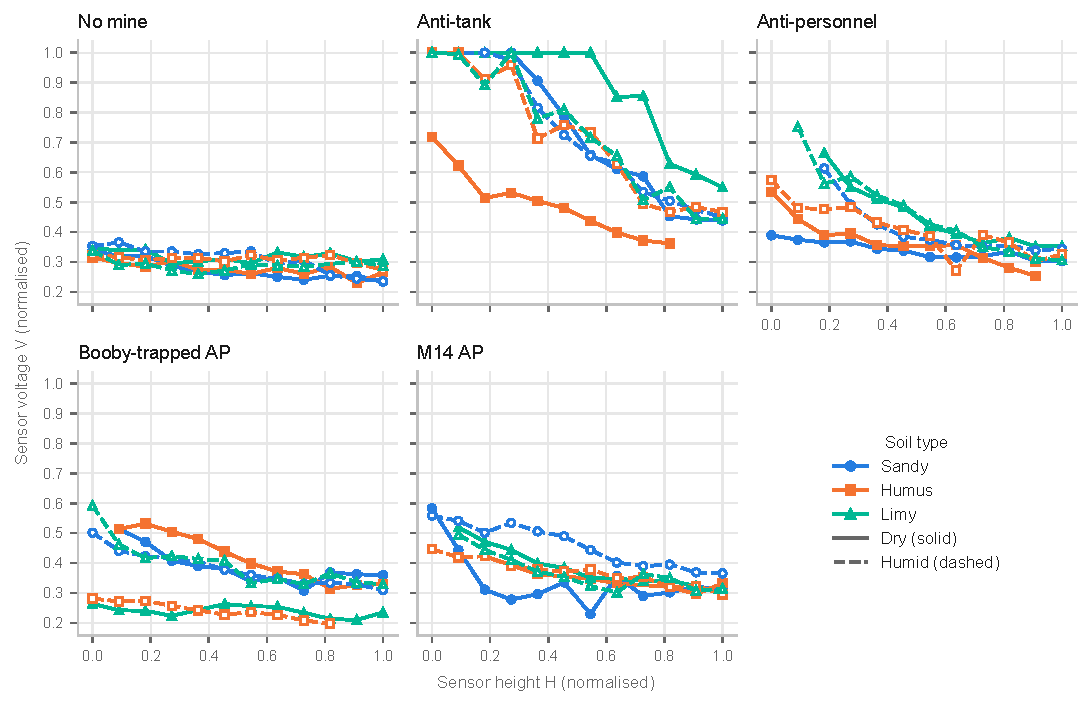
\includegraphics[width=\columnwidth]{fig05_voltage_vs_height_by_class.pdf}
\caption{Voltage against sensor height for each class (one line per soil). Signals decay with height; anti-tank mines saturate the sensor close to the ground, and the three anti-personnel types overlap strongly.}
\label{fig:eda}
\end{figure}

\section{Methodology}
\subsection{Physics-informed inputs}
All neural models receive the raw $(V,H)$ and the soil index; feature construction is part of the network, so the exported model needs no external preprocessing. The physics feature layer computes an effective distance $r=H+d_0$, where $d_0$ is fitted on the training rows of each split by minimising the residual of the inverse-cube model above (closed form for $a,b$; grid search for $d_0$; saturated readings excluded), and a soil background $b(S)$, the mean no-mine voltage of that soil in the training rows. It adds $\log V$, $Vr^3$, $V/r$, the distance-compensated anomaly $(V-b(S))\,r^3$ and a saturation flag. All features are standardised with training statistics.

\subsection{Architectures}
The \textbf{MLP} concatenates the features with a learned soil embedding and applies 1--3 blocks of linear layer, batch normalisation~\cite{ioffe2015}, ReLU and dropout~\cite{srivastava2014}. The \textbf{FT-Transformer}~\cite{gorishniy2021} maps every numeric feature $x_i$ to a token $x_i w_i + b_i$, adds a soil-embedding token and a [CLS] token, and applies 1--3 pre-norm Transformer blocks; the final [CLS] state is classified (Fig.~\ref{fig:arch}). ``+ physics features'' variants use the physics layer; ``PI'' (physics-informed) variants also use the consistency loss below.

\begin{figure*}[t]
\centering
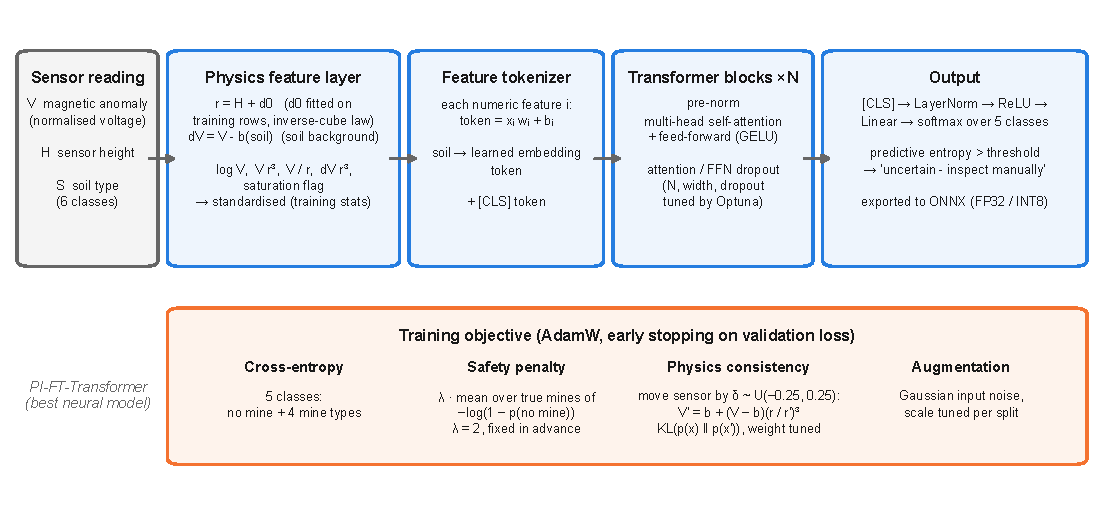
\includegraphics[width=\textwidth]{fig00_architecture.pdf}
\caption{The physics-informed FT-Transformer (\pift) and its training objective.}
\label{fig:arch}
\end{figure*}

\subsection{Training objective}
The loss is
\begin{equation}
\mathcal{L} = \mathrm{CE} + \lambda_{s}\,\frac{1}{n}\!\sum_{i:\,y_i\neq 0}\!-\log\!\big(1-p_0(x_i)\big) + \lambda_{p}\,\mathrm{KL}\big(\bar p(x)\,\|\,p(x')\big),
\end{equation}
where $p_0$ is the predicted probability of ``no mine''. The second term is a cost-sensitive safety penalty that grows without bound as the model becomes confident that a real mine is empty ground; $\lambda_s=2$ was fixed before any experiment and never tuned on test data. The third term is a physics-consistency loss: each reading is moved to a new height $H'=H+\delta$, $\delta\sim U(-0.25,0.25)$, and its anomaly is rescaled by the inverse-cube law, $V'=b+(V-b)\,(r/r')^3$; the model must predict the same class distribution for $x'$ as for $x$ (with the target $\bar p(x)$ detached, and saturated readings excluded). Inputs are augmented with Gaussian noise whose scale, a multiple of each input's training standard deviation, is tuned. Models are trained with AdamW~\cite{loshchilov2019} and early stopping on validation cross-entropy.

\subsection{Uncertainty}
MC dropout~\cite{gal2016} averages 50 stochastic passes. A reading is flagged ``uncertain -- inspect manually'' if its predictive entropy exceeds the 80th percentile of the entropy on the split's validation rows; the threshold is fixed before the test fold is seen. Temperature scaling~\cite{guo2017} is fitted on the same validation rows.

\section{Experimental Setup}
\textbf{Protocol.} Outer loop: stratified 5-fold CV repeated with 5 seeds, giving 25 test folds of \vTestFoldMin--\vTestFoldMax{} readings; every model sees identical splits, so all comparisons are paired. A stratified 15\,\% of each outer training part is held out for early stopping (e.g.\ \vTrainFirst{} training and \vValFirst{} validation rows in the first split). Inner loop: Optuna~\cite{akiba2019} with the TPE sampler~\cite{bergstra2011} and median pruning maximises macro-F1 over 3 stratified folds of the outer training rows (40 trials for neural models, 60 for baselines). The outer test fold is used once, for scoring.

\textbf{Baselines.} $k$-NN, an RBF SVM~\cite{cortes1995} with Platt scaling~\cite{platt1999}, random forest~\cite{breiman2001} and XGBoost~\cite{chen2016}, implemented with scikit-learn~\cite{pedregosa2011}, all with soil one-hot encoded and the same nested tuning. A first SVM search capped $C$ at $10^3$ and the tuned values reached that cap; we widened the range to $[10^{-2},10^5]$ (median tuned $C=\vSvmCMedian$) and report the wider search, which scored \vAccSvm{} against \vAccSvmNarrow{} for the narrower one.

\textbf{Statistics.} Per-split scores of repeated CV are dependent, so in addition to the Wilcoxon signed-rank test~\cite{wilcoxon1945} we report the corrected repeated $k$-fold $t$-test~\cite{nadeau2003,bouckaert2004}, which inflates the variance by $n_\text{test}/n_\text{train}$, and the exact McNemar test~\cite{mcnemar1947} within each seed. Families of comparisons are Holm-corrected~\cite{holm1979}. We call a difference significant only if the corrected $t$-test gives $p<0.05$.

\textbf{Leakage check.} Re-running SVM, PI-MLP and \pift{} with training labels shuffled gives \vPermMin--\vPermMax\,\% mean accuracy, the chance level for five classes.

\textbf{Implementation.} PyTorch~\cite{paszke2019}, CPU training with fixed seeds. On the development laptop, CPU training was faster than Apple's MPS backend for these small models (FT-Transformer: \vDevFtCpu\,s vs.\ \vDevFtMps\,s per 100 epochs).

\section{Results}
\subsection{Accuracy and safety}
Table~\ref{tab:main} and Fig.~\ref{fig:cv} summarise the nested CV. The SVM has the highest mean accuracy (\vAccSvm) and the lowest false-alarm rate; \pift{} is the best neural model (\vAccPiFt). Their difference (\vDiffPiFtVsSvmAccuracy{} points) is not significant (Table~\ref{tab:sig}); \pift{} is significantly more accurate than random forest, XGBoost and $k$-NN. All neural models miss fewer mines than every baseline (\vMissPiFt\,\% for \pift, \vMissSvm\,\% for the SVM) at the cost of more false alarms (\vFaPiFt\,\% vs.\ \vFaSvm\,\%), as intended by the safety loss; the mine-missed difference to the SVM is not significant under the corrected test ($p$~\vPtPiFtVsSvmMineMissed). The FT-Transformer is more accurate than the MLP by a margin that is suggestive but not significant ($p$~\vPtFtVsMlpAccuracy). Mine versus no-mine detection accuracy is about \vDetPiFt\,\% for \pift{} and \vDetSvm\,\% for the SVM. All models confuse the three anti-personnel types (Fig.~\ref{fig:cm}), whose signals overlap (Fig.~\ref{fig:eda}).

\begin{table}[t]
\centering
\caption{Nested-CV results (mean over 25 test folds; accuracy $\pm$ std). Det.: mine vs.\ no-mine accuracy; Miss: share of real mines predicted as no mine; FA: share of empty readings predicted as a mine (all in \%).}
\label{tab:main}
\setlength{\tabcolsep}{2.5pt}
\scriptsize
\begin{tabular}{lccccc}
\toprule
Model & Accuracy & Macro F1 & Det. & Miss & FA \\
\midrule
% Generated from results/. Do not edit.
\textbf{PI-FT-Transformer} & 0.703 $\pm$ 0.052 & 0.693 & 92.4 & 4.0 & 20.9 \\
FT-Transformer & 0.692 $\pm$ 0.049 & 0.682 & 92.8 & 4.2 & 18.6 \\
FT-Transformer + phys. features & 0.691 $\pm$ 0.059 & 0.685 & 92.0 & 3.6 & 24.5 \\
PI-MLP & 0.676 $\pm$ 0.062 & 0.669 & 91.8 & 3.3 & 26.5 \\
MLP + phys. features & 0.667 $\pm$ 0.056 & 0.661 & 91.5 & 3.6 & 27.1 \\
MLP & 0.648 $\pm$ 0.055 & 0.643 & 91.4 & 2.1 & 33.0 \\
\midrule
SVM (RBF) & 0.719 $\pm$ 0.057 & 0.706 & 93.1 & 5.8 & 11.3 \\
Random forest & 0.591 $\pm$ 0.048 & 0.576 & 90.6 & 7.3 & 17.5 \\
XGBoost & 0.539 $\pm$ 0.054 & 0.523 & 88.6 & 8.5 & 22.4 \\
k-NN & 0.439 $\pm$ 0.055 & 0.421 & 78.8 & 15.7 & 41.7 \\
\bottomrule

\end{tabular}
\end{table}

\begin{table}[t]
\centering
\caption{\pift{} minus each baseline, paired over 25 folds (difference in percentage points; W/T/L = folds where \pift{} is higher/tied/lower). Holm-corrected $p$-values.}
\label{tab:sig}
\setlength{\tabcolsep}{3pt}
\footnotesize
\begin{tabular}{llcccc}
\toprule
Baseline & Metric & Diff. & W/T/L & Wilcoxon & Corr.\ $t$ \\
\midrule
% Generated from results/. Do not edit.
k-NN & accuracy & +26.5 & 25/0/0 & $<$\,0.001 & $<$\,0.001 \\
k-NN & mines missed & $-$11.7 & 0/0/25 & $<$\,0.001 & 0.0091 \\
SVM (RBF) & accuracy & $-$1.6 & 9/3/13 & 0.33 & 0.66 \\
SVM (RBF) & mines missed & $-$1.7 & 5/4/16 & 0.0073 & 0.27 \\
Random forest & accuracy & +11.2 & 24/1/0 & $<$\,0.001 & 0.0017 \\
Random forest & mines missed & $-$3.2 & 2/3/20 & $<$\,0.001 & 0.20 \\
XGBoost & accuracy & +16.4 & 25/0/0 & $<$\,0.001 & $<$\,0.001 \\
XGBoost & mines missed & $-$4.5 & 2/1/22 & $<$\,0.001 & 0.17 \\
\bottomrule

\end{tabular}
\end{table}

\begin{figure*}[t]
\centering
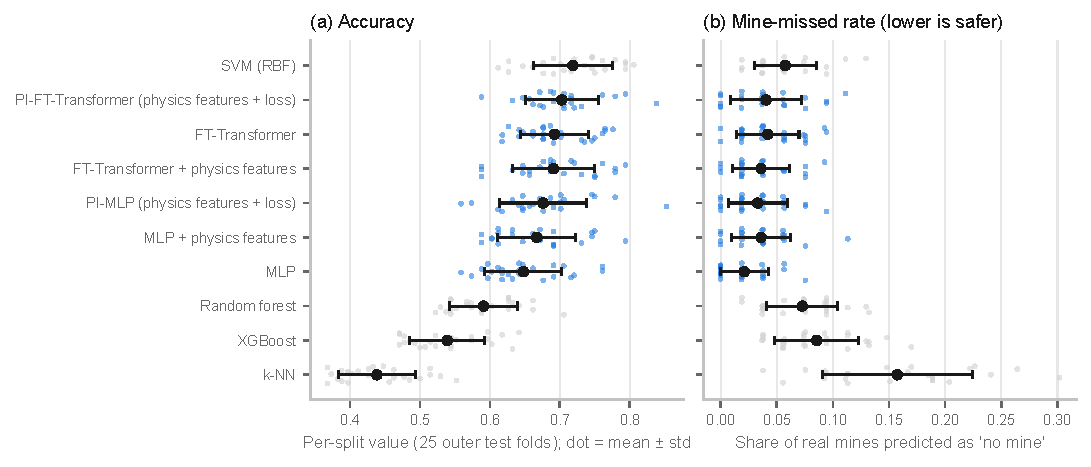
\includegraphics[width=\textwidth]{fig08_nested_cv_results.pdf}
\caption{Per-fold accuracy and mine-missed rate for every model (dots: the 25 test folds; black: mean $\pm$ std). Neural models in blue.}
\label{fig:cv}
\end{figure*}

\begin{figure*}[t]
\centering
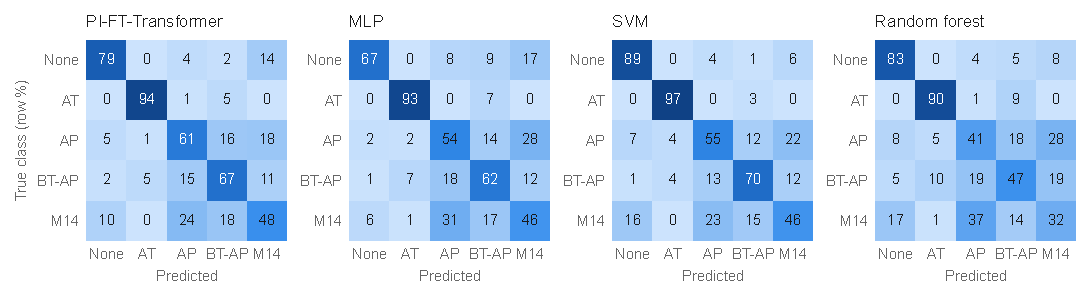
\includegraphics[width=\textwidth]{fig10_confusion_matrices.pdf}
\caption{Row-normalised confusion matrices pooled over all test folds (\%).}
\label{fig:cm}
\end{figure*}

\subsection{Physics}\label{sec:physics}
Physics features plus the consistency loss raised accuracy by \vPhysgainPiMlpVsMlp{} points for the MLP (better in \vPhysbetterPiMlpVsMlp{} of 25 folds, worse in \vPhysworsePiMlpVsMlp) and by \vPhysgainPiFtVsFt{} points for the FT-Transformer (\vPhysbetterPiFtVsFt{} better, \vPhysworsePiFtVsFt{} worse). Neither gain is significant ($p$~\vPtPiMlpVsMlpAccuracy{} and $p$~\vPtPiFtVsFtAccuracy). The fitted offset $d_0$ had a median of \vDZeroMedian{} (range \vDZeroMin--\vDZeroMax) across splits: the effective distance is dominated by the offset, so over the measured heights the inverse-cube curve is close to linear and the physics features carry little information that a network cannot learn from $H$ directly.

\subsection{Uncertainty and calibration}
Table~\ref{tab:unc} and Fig.~\ref{fig:rel} report calibration and the uncertainty flag. The raw \pift{} is reasonably calibrated (ECE \vEcePiFt, SVM \vEceSvm). Temperature scaling did not improve calibration for any neural model and made it slightly \emph{worse} for most (\pift: \vEcetsPiFt): its temperature is fitted on few validation rows (\vValFirst{} in the first split) that early stopping has already used. MC-dropout averaging improved ECE for the FT-Transformer models (\pift: \vEcemcPiFt). The 80th-percentile flag marks \vUncPiFtMcFlaggedShare\,\% of readings; accuracy is \vUncPiFtMcAccuracyConfident\,\% on the rest and \vUncPiFtMcAccuracyFlagged\,\% on flagged readings, and only \vUncPiFtMcMineMissedUnflagged\,\% of mines are missed without a flag. A single deterministic pass ranks readings as well as 50 MC-dropout passes (area under the risk--coverage curve \vUncPiFtSmAurc{} vs.\ \vUncPiFtMcAurc), so the deployed model uses the one-pass entropy.

Ranking by confidence is where \pift{} clearly differs from the SVM (Fig.~\ref{fig:rc}): when only the 50\,\% most confident readings are decided automatically, \pift{} is correct on \vSelPiFtMcFifty\,\% and the SVM on \vSelSvmMpFifty\,\% (\vSelwinsSvmAccAtFiveZero{} wins, \vSellossesSvmAccAtFiveZero{} losses; Wilcoxon $p$~\vSelpwSvmAccAtFiveZero, corrected $p$~\vSelpSvmAccAtFiveZero). The conservative test does not reach significance, so this is strong but not conclusive evidence.

\begin{table*}[t]
\centering
\caption{Calibration (ECE, lower is better) and the ``inspect manually'' flag. Flag columns: accuracy on unflagged and flagged readings with MC dropout, accuracy on unflagged readings with the one-pass entropy flag, and the share of mines missed without a flag (one-pass). All flags refer about 20\,\% of readings.}
\label{tab:unc}
\footnotesize
\begin{tabular}{lccccccc}
\toprule
 & \multicolumn{3}{c}{ECE} & \multicolumn{2}{c}{MC-dropout flag (\%)} & \multicolumn{2}{c}{One-pass flag (\%)} \\
Model & raw & temp.\ scaled & MC dropout & acc.\ unflagged & acc.\ flagged & acc.\ unflagged & mines missed, unflagged \\
\midrule
% Generated from results/. Do not edit.
PI-FT-Transformer & 0.060 & 0.068 & 0.050 & 77.7 & 40.7 & 77.2 & 3.1 \\
FT-Transformer & 0.055 & 0.065 & 0.049 & 75.1 & 41.9 & 76.3 & 3.7 \\
PI-MLP & 0.064 & 0.071 & 0.065 & 73.4 & 43.4 & 73.9 & 2.1 \\
MLP & 0.054 & 0.075 & 0.047 & 70.9 & 35.7 & 71.4 & 1.5 \\
SVM (RBF) & 0.078 & -- & -- & -- & -- & -- & -- \\
Random forest & 0.070 & -- & -- & -- & -- & -- & -- \\
\bottomrule

\end{tabular}
\end{table*}

\begin{figure*}[t]
\centering
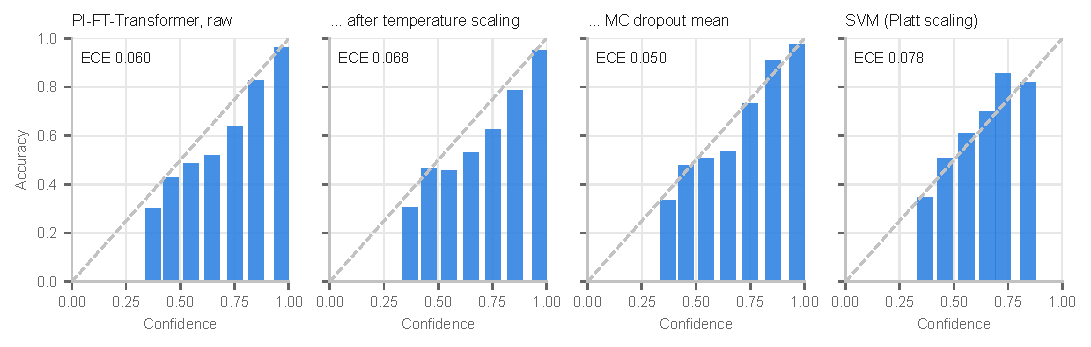
\includegraphics[width=\textwidth]{fig12_reliability_diagrams.pdf}
\caption{Reliability diagrams pooled over all test folds; ECE is the mean over the five repetitions.}
\label{fig:rel}
\end{figure*}

\begin{figure}[t]
\centering
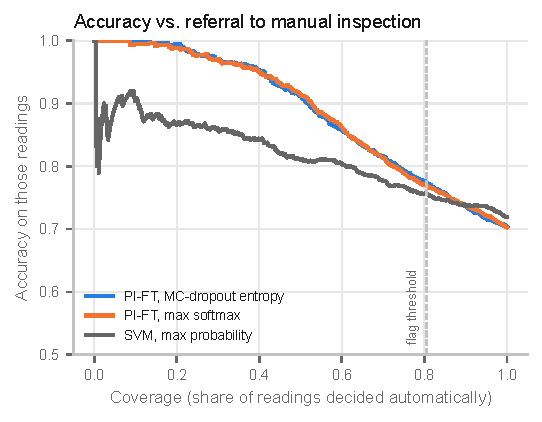
\includegraphics[width=0.92\columnwidth]{fig13_risk_coverage.pdf}
\caption{Accuracy on the most confident readings as a function of coverage. The dashed line marks the deployed flag threshold.}
\label{fig:rc}
\end{figure}

\subsection{Robustness to sensor noise}
Adding Gaussian noise to $V$ and $H$ at test time degrades every model (Fig.~\ref{fig:noise}). Accuracy falls at similar rates for \pift{} and the SVM, but the SVM increasingly calls mines empty ground: at a noise level of 0.5 training standard deviations, \pift{} misses \vNoisePiFtHalfMiss\,\% of mines and the SVM \vNoiseSvmHalfMiss\,\% (fewer misses in \vNoiselossesHalfMineMissed{} of 25 folds; corrected $p$~\vNoisepHalfMineMissed, Holm-corrected over the 8 noise levels $p$~\vNoiseHolmHalf). The difference remains significant after this correction for every noise level from \vNoiseHolmMinSigma{} upwards.

\begin{figure*}[t]
\centering
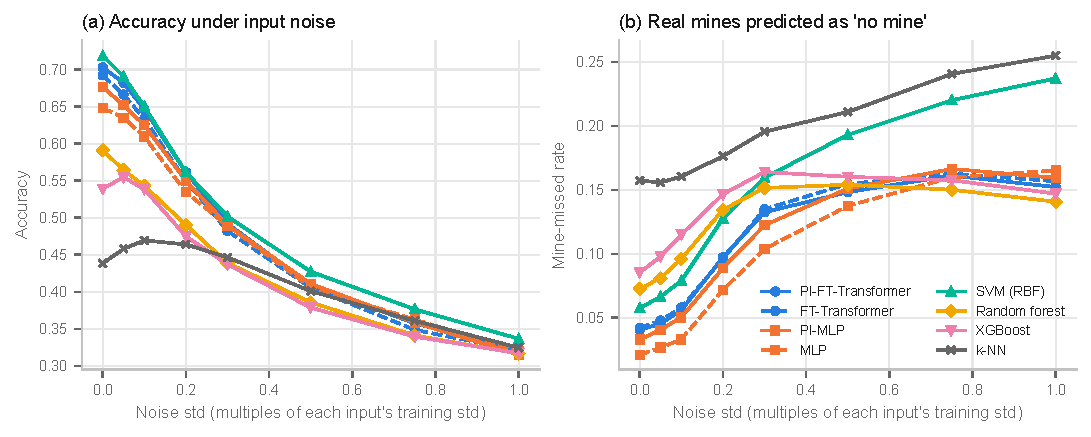
\includegraphics[width=\textwidth]{fig14_noise_robustness.pdf}
\caption{Accuracy and mine-missed rate under test-time Gaussian noise (mean over 25 folds, 5 noise draws each).}
\label{fig:noise}
\end{figure*}

\subsection{Unseen soils}
Leave-one-soil-out evaluation (train on five soils, test on the sixth; hyperparameters tuned by an inner leave-one-soil-out loop) shows that no model generalises to a new soil (Table~\ref{tab:loso}): accuracy drops from the levels of the main CV (column ``Seen'') to \vLosoMin--\vLosoMax\,\%. The best results come from an MLP that ignores soil (\vLosopctMlpNone\,\%) and from the SVM (\vLosopctSvm\,\%); factorising soil into moisture and texture embeddings did not help. Dry humus is the hardest held-out soil on average and for every model except the SVM (\vLosoDryHumusMin--\vLosoDryHumusMax\,\% across models).

\begin{table}[t]
\centering
\caption{Leave-one-soil-out (mean over held-out soils, $\pm$ std over 5 refits). Miss in \%. ``Seen'': accuracy of the same model family in the main CV, where every soil is seen in training.}
\label{tab:loso}
\setlength{\tabcolsep}{2.5pt}
\scriptsize
\begin{tabular}{lccc}
\toprule
Model & Accuracy & Miss & Seen \\
\midrule
% Generated from results/. Do not edit.
MLP, no soil input & 0.428 $\pm$ 0.014 & 5.2 & 0.646 \\
k-NN & 0.426 $\pm$ 0.000 & 25.4 & 0.436 \\
MLP, soil embedding (mean vector for unseen soil) & 0.418 $\pm$ 0.027 & 10.3 & 0.646 \\
SVM (RBF) & 0.406 $\pm$ 0.010 & 20.6 & 0.717 \\
Random forest & 0.398 $\pm$ 0.003 & 20.8 & 0.588 \\
XGBoost & 0.397 $\pm$ 0.012 & 21.1 & 0.536 \\
PI-FT-Transformer, factorised soil embedding & 0.396 $\pm$ 0.027 & 15.5 & 0.701 \\
FT-Transformer, factorised soil embedding & 0.367 $\pm$ 0.037 & 17.1 & 0.689 \\
MLP, factorised soil embedding & 0.367 $\pm$ 0.029 & 13.3 & 0.646 \\
PI-MLP, factorised soil embedding & 0.348 $\pm$ 0.043 & 15.7 & 0.674 \\
\bottomrule

\end{tabular}
\end{table}

\subsection{Explanations}
Exact Shapley values~\cite{lundberg2017} (three inputs, so all $2^3$ coalitions are evaluated) show that $V$ carries \vShapvPiFt\,\% of the total attribution for \pift, $H$ \vShaphPiFt\,\% and soil \vShapsPiFt\,\%; the SVM's attributions are similar (\vShapvSvm/\vShaphSvm/\vShapsSvm\,\%). Relative to $V$, soil carries much more weight for the three anti-personnel types than for anti-tank mines, whose strong signals need little context (Fig.~\ref{fig:shap}). Per-prediction explanations make individual failures visible; the missed mine shown in the figure is an anti-personnel reading whose low voltage pushes the model towards ``no mine''.

\begin{figure*}[t]
\centering
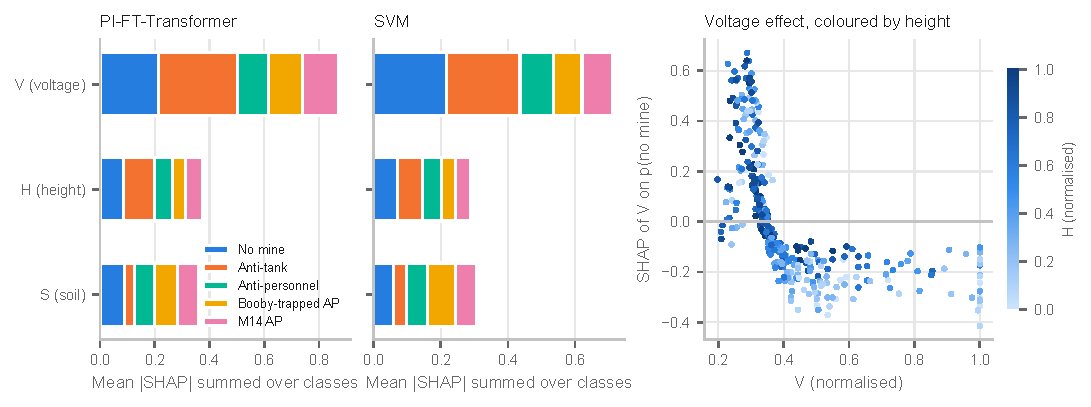
\includegraphics[width=\textwidth]{fig15_shap_global.pdf}\\[2pt]
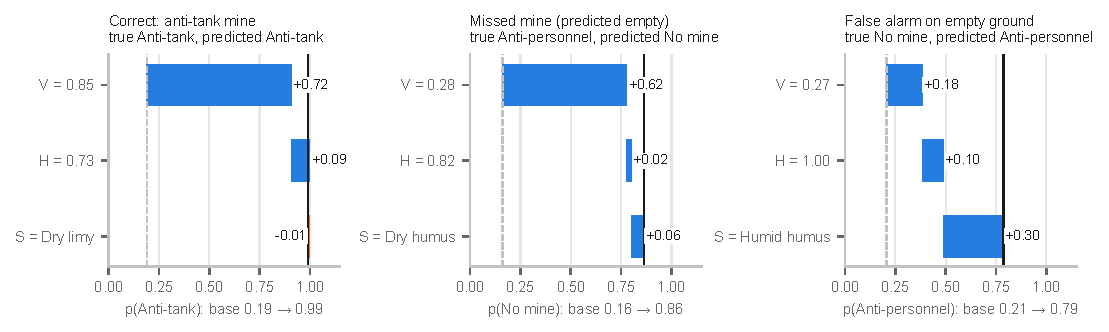
\includegraphics[width=\textwidth]{fig18_shap_local.pdf}
\caption{SHAP explanations. Top: mean $|\text{SHAP}|$ per input, stacked by class, and the effect of $V$ on $p(\text{no mine})$. Bottom: three individual \pift{} predictions (dashed: average prediction; solid: this reading).}
\label{fig:shap}
\end{figure*}

\subsection{Edge deployment}
The deployed \pift{} is the same tuning procedure applied to all readings (inner macro-F1 \vFinalInnerFOne; \vFinalBlocks{} blocks of width \vFinalDtoken; \vEdgeParams{} parameters). Exported to ONNX it matches PyTorch to \vParityFpThreeTwo; dynamic INT8 quantisation shrinks it to \vEdgeKbIntEight~KB and agrees with the full-precision model on \vParityIntEightAgree\,\% of 20{,}000 random readings (\vParityIntEightFlag\,\% for the flag). On one CPU thread of the development laptop a single reading takes about \vLatOnnxIntEight~\textmu s (Table~\ref{tab:edge}); quantisation saves memory but not time at this size. These timings are not from an embedded board; they suggest that real-time use on handheld or drone hardware is plausible, which remains to be measured.

\begin{table}[t]
\centering
\caption{Size and speed of the deployed model (one CPU thread, development laptop).}
\label{tab:edge}
\footnotesize
\setlength{\tabcolsep}{3pt}
\begin{tabular}{lccc}
\toprule
Runtime & Size (KB) & 1 reading (\textmu s) & Readings/s \\
\midrule
% Generated from results/. Do not edit.
PyTorch (eager) & 279 & 132 & 70,208 \\
ONNX Runtime, FP32 & 283 & 78 & 68,113 \\
ONNX Runtime, INT8 & 101 & 76 & 63,214 \\
\bottomrule

\end{tabular}
\end{table}

\subsection{Comparison with the original study}
Table~\ref{tab:bench} places our results next to those of~\cite{yilmaz2018}. The protocols differ: a single split of 113 test readings, with test data used inside the meta-heuristic's fitness, against nested CV over 25 test folds. Our single-fold accuracies span a wide range (e.g.\ \vAccminPiFt--\vAccmaxPiFt\,\% for \pift), so a single small split can land far above or below the mean; we therefore do not claim to beat or fall short of the published figures.

\begin{table}[t]
\centering
\caption{Comparison with Yilmaz et al.~\cite{yilmaz2018}. Brackets: range over single test folds.}
\label{tab:bench}
\setlength{\tabcolsep}{2.5pt}
\scriptsize
\begin{tabular}{lccc}
\toprule
Model & Protocol & 5-class acc. & Detection \\
\midrule
% Generated from results/. Do not edit.
Meta-heuristic $k$-NN \cite{yilmaz2018} & single split, 113 test & 85.8\,\% & 98.2\,\% \\
ANN \cite{yilmaz2018} & single split, 113 test & 71.3\,\% & -- \\
\midrule
SVM (RBF) (ours) & nested CV, 25 folds & 71.9\,\% [61.2--80.6] & 93.1\,\% \\
PI-FT-Transformer (ours) & nested CV, 25 folds & 70.3\,\% [58.8--83.8] & 92.4\,\% \\
FT-Transformer (ours) & nested CV, 25 folds & 69.2\,\% [61.8--77.6] & 92.8\,\% \\
PI-MLP (ours) & nested CV, 25 folds & 67.6\,\% [55.9--85.3] & 91.8\,\% \\
Random forest (ours) & nested CV, 25 folds & 59.1\,\% [52.2--70.6] & 90.6\,\% \\
\bottomrule

\end{tabular}
\end{table}

\section{Ablation Study}
Each component was removed in turn from PI-MLP and \pift, reusing the hyperparameters tuned for each split in the main experiment and retraining with the same seeds (the full models reproduced the main results exactly). Removing an input means replacing it with its training mean. Table~\ref{tab:ablation} and Fig.~\ref{fig:ablation} report the change in accuracy.

\begin{table}[t]
\centering
\caption{Ablation: change in accuracy (percentage points) and corrected $t$-test $p$-value, paired over 25 folds.}
\label{tab:ablation}
\setlength{\tabcolsep}{3pt}
\scriptsize
\begin{tabular}{lcccc}
\toprule
 & \multicolumn{2}{c}{PI-MLP} & \multicolumn{2}{c}{\pift} \\
Removed & $\Delta$ & $p$ & $\Delta$ & $p$ \\
\midrule
% Generated from results/. Do not edit.
no $V$ input & $-$50.1 & $<$\,0.001 & $-$51.5 & $<$\,0.001 \\
no $H$ input & $-$19.9 & $<$\,0.001 & $-$21.8 & $<$\,0.001 \\
no soil input & $-$8.1 & 0.0048 & $-$13.4 & $<$\,0.001 \\
no physics features & $-$2.4 & 0.49 & $-$1.8 & 0.49 \\
no physics loss & $-$1.1 & 0.64 & $-$1.8 & 0.51 \\
no physics at all & $-$3.1 & 0.30 & $-$2.0 & 0.52 \\
no noise augmentation & +0.8 & 0.77 & +0.7 & 0.82 \\
no batch norm & +3.9 & 0.18 & n/a &  \\
no dropout & $-$0.7 & 0.75 & $-$0.1 & 0.98 \\
one-hot soil (no embedding) & +0.5 & 0.84 & n/a &  \\
\bottomrule

\end{tabular}
\end{table}

\begin{figure*}[t]
\centering
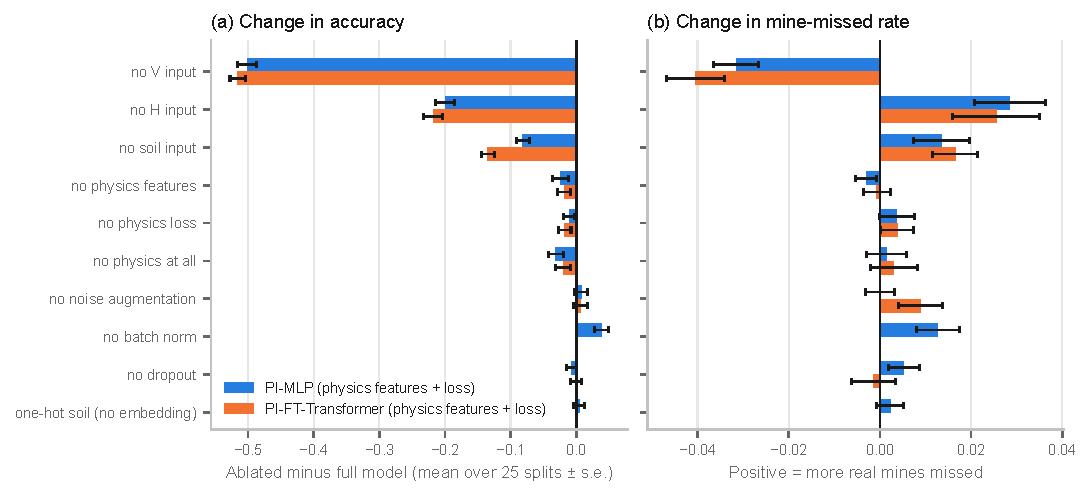
\includegraphics[width=0.85\textwidth]{fig16_ablation.pdf}
\caption{Ablation: change against the full model (mean over 25 folds $\pm$ standard error).}
\label{fig:ablation}
\end{figure*}

\begin{figure}[t]
\centering
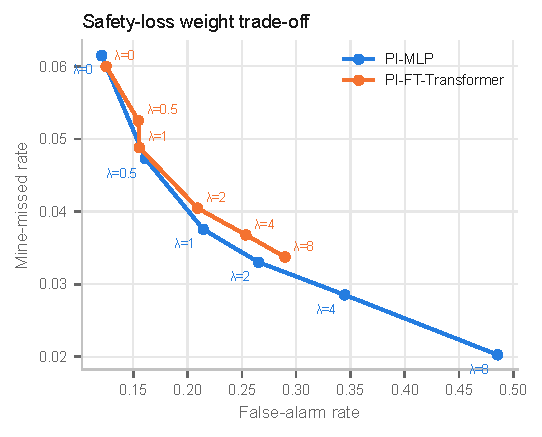
\includegraphics[width=0.8\columnwidth]{fig17_safety_tradeoff.pdf}
\caption{Missed mines against false alarms as the safety-loss weight $\lambda_s$ varies.}
\label{fig:safety}
\end{figure}

The inputs dominate: without $V$ accuracy collapses to about chance, and removing $H$ or soil changes the accuracy of \pift{} by \vAbPiFtNoh{} and \vAbPiFtNosoil{} points. Removing the physics features (\vAbPiFtNophysfeat), the physics loss (\vAbPiFtNophysloss) or both (\vAbPiFtNophys) lowers accuracy slightly but not significantly, consistent with Section~\ref{sec:physics}. Dropout, noise augmentation and the soil embedding (versus one-hot) make no measurable difference; the tuned noise scale sat near the lower edge of its search range. Removing batch normalisation \emph{improved} the PI-MLP by \vAbPiMlpNobn{} points (Wilcoxon $p$~\vAbpwPiMlpNobn, corrected $p$~\vAbpPiMlpNobn), even though the reused hyperparameters were tuned with batch normalisation; with only \vTrainFirst{} training rows per split and batches of 32, batch statistics are noisy.

The safety weight trades missed mines against false alarms (Fig.~\ref{fig:safety}): for \pift, $\lambda_s=0$ gives \vSwPiFtZeroMiss\,\% missed mines and \vSwPiFtZeroFa\,\% false alarms, $\lambda_s=2$ gives \vSwPiFtTwoMiss\,\% and \vSwPiFtTwoFa\,\%, and $\lambda_s=8$ gives \vSwPiFtEightMiss\,\% and \vSwPiFtEightFa\,\%; accuracy changes little (\vSwPiFtZeroAcc{} to \vSwPiFtEightAcc). The weight is therefore an operating-point choice for the user, not a free improvement.

\section{Discussion}
\textbf{Deep learning versus a tuned SVM.} On \vRows{} readings of three inputs, a well-tuned kernel machine is as accurate as the best neural model. The neural model's advantages lie elsewhere: confidence that ranks readings better, more graceful degradation under noise with respect to missed mines, an objective that encodes the asymmetric cost of errors, and a single differentiable pipeline that includes the physics and exports to a \vEdgeKbIntEight-KB edge model.

\textbf{Physics.} The inverse-cube model describes the data well ($R^2=\vEdaRTwoCube$), but the fitted offset is larger than the measured height range, so physics-based features add little beyond what the network learns from $H$. A sensor sweep over a wider range of heights, or data in physical units, would test the idea more sharply.

\textbf{Limitations.} The dataset is small and comes from one experimental set-up; each (soil, height, class) combination is observed once, so test readings are always new combinations rather than repeated measurements. No model transfers to an unseen soil. The edge timings are from a laptop. The minefield demonstrator uses synthetic readings from the fitted inverse-cube model and is not an evaluation.

\section{Conclusion}
MineSense combines a physics-informed FT-Transformer, a safety-aware objective and an explicit uncertainty flag. Under nested cross-validation it is statistically tied with a tuned SVM in accuracy (\vAccPiFt{} vs.\ \vAccSvm), better than tree ensembles and $k$-NN, ranks its own confidence better, and misses fewer mines under sensor noise; its INT8 model is \vEdgeKbIntEight~KB. Physics-based features and loss help only slightly here, and transfer to new soils remains open. We hope the protocol, the negative results and the released pipeline make future comparisons on this dataset easier to trust.

\bibliographystyle{IEEEtran}
\bibliography{references}

\end{document}
